\documentclass[10pt]{beamer}

\usetheme{metropolis}
\usepackage{appendixnumberbeamer}

\usepackage{graphicx}
\graphicspath{ {../img/} }

\usepackage{multirow}
\usepackage{booktabs} % Allows the use of \toprule, \midrule and \bottomrule in tables
\newcommand{\tabitem}{~~\llap{\textbullet}~~}
\usepackage[scale=2]{ccicons}

\usepackage{pgfplots}
\usepgfplotslibrary{dateplot}

\usepackage{xspace}
\newcommand{\themename}{\textbf{\textsc{metropolis}}\xspace}

\usepackage{tikz}
\usetikzlibrary{shapes.geometric, arrows, fit, positioning, calc}
\tikzstyle{data} = [rectangle, rounded corners, minimum width=2.5cm, minimum height=0.8cm, text centered, text width=2.5cm, draw=black, fill=blue!30]

\usepackage{relsize}
\tikzset{fontscale/.style = {font=\relsize{#1}}}

\usepackage{color}
\newcommand{\tc}[1]{\textcolor{red}{#1}}

%----------------------------------------------------------------------------------------
% TITLE PAGE
%----------------------------------------------------------------------------------------
\title[Interface of 3D Reconstruction]{Development and Application of a Description-based Interface for 3D Reconstruction} % The short title appears at the bottom of every slide, the full title is only on the title page

\author{Kai Wu}
\institute[UBC]
{
University of British Columbia \\ % Your institution for the title page
\medskip
kaywu@ece.ubc.ca \\ % Your email address
}
\date{\today}

\begin{document}

\begin{frame}
\maketitle
\end{frame}

\begin{frame}{Table of contents}
  \setbeamertemplate{section in toc}[sections numbered]
  \tableofcontents[hideallsubsections]
\end{frame}


%------------------------------------------------
\section{Additional Slides}
%------------------------------------------------
\begin{frame}{Description: expression}

We use three-scale values to parameterize properties: \textit{low} (0.2), \textit{medium} (0.5), and \textit{high} (0.8).

\begin{figure}[!htbp]
\centering
\begin{tabular}{cccc}
  \includegraphics[width=0.25\textwidth]{images/desc_vase.pdf}&
  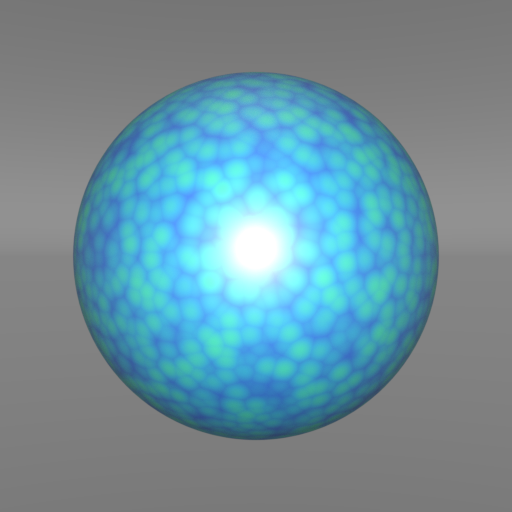
\includegraphics[width=0.2\textwidth]{interp/ui/ui_sphere.png}&
  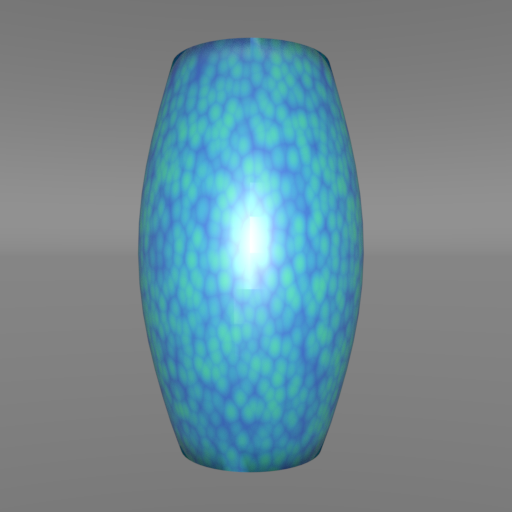
\includegraphics[width=0.2\textwidth]{interp/ui/ui_vase.png}&
  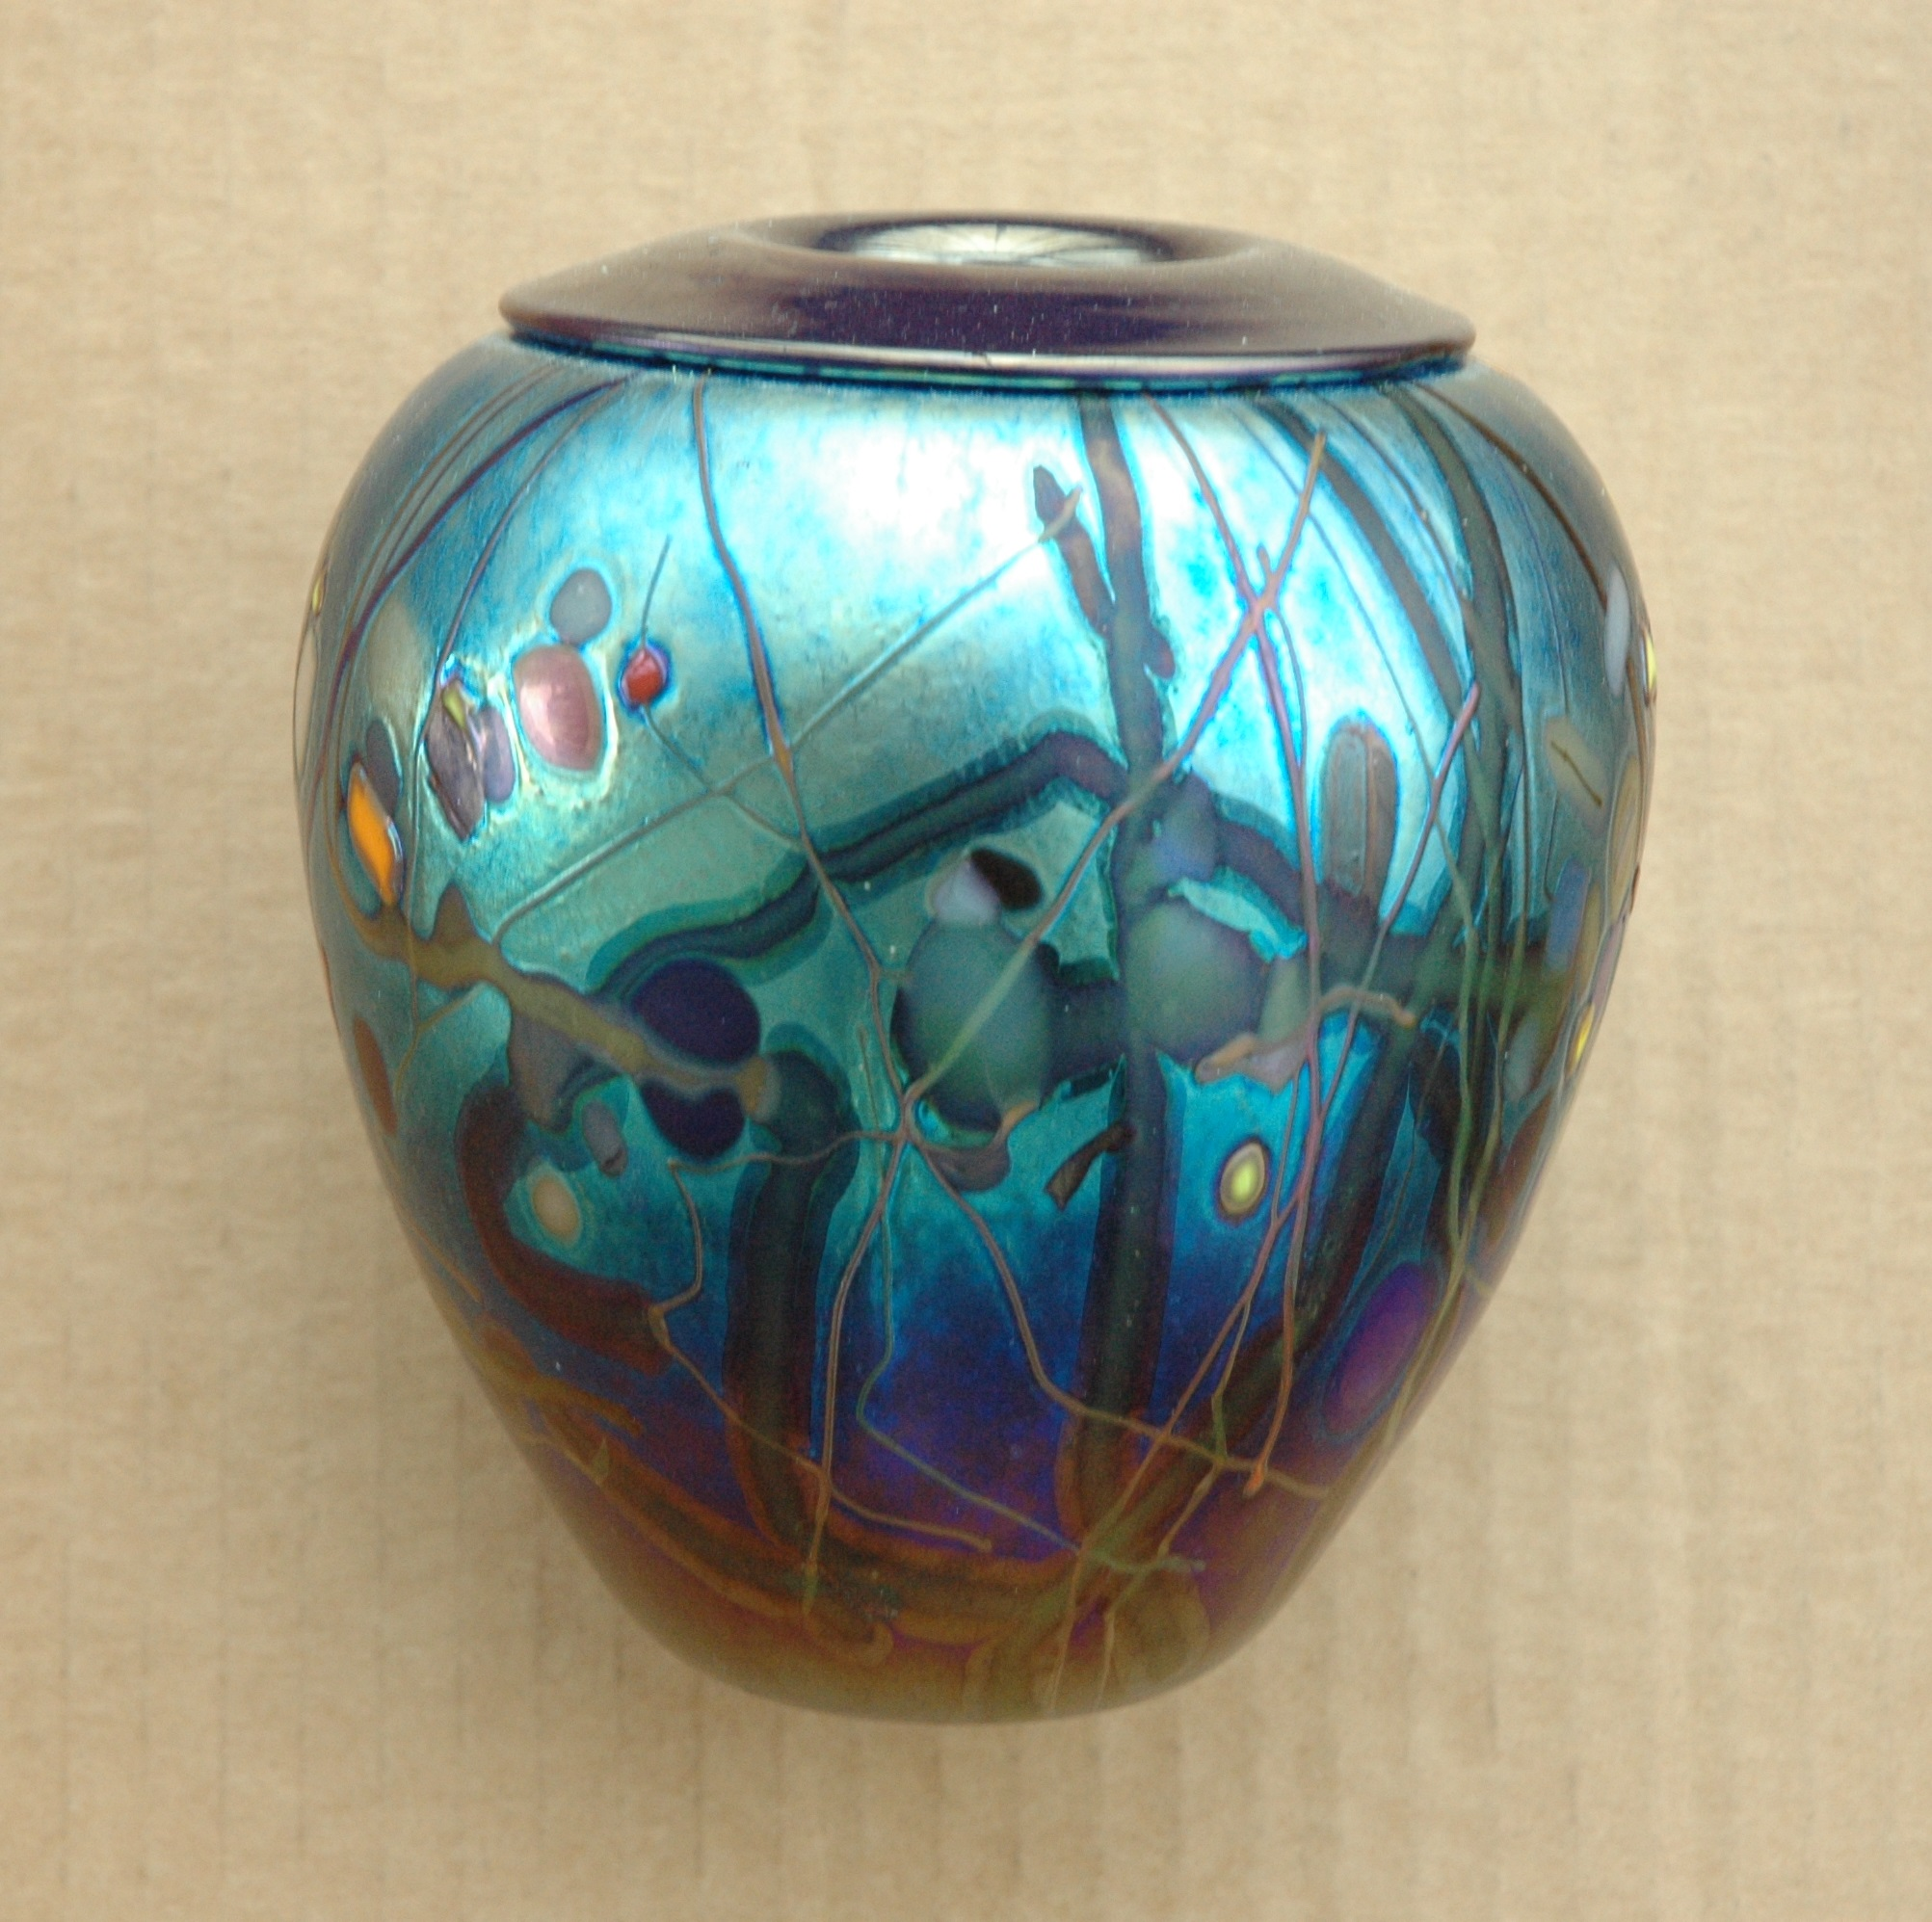
\includegraphics[width=0.2\textwidth]{interp/real_world_img/vase/vase.jpg}\\
  Property settings & Synthetic sphere & Synthetic vase & Real-world vase\\
\end{tabular}
% \caption{(a) demonstrates the effect of the property settings on a sphere, (b) on a teapot, and (c) shows the real-world object.}
\end{figure}

\end{frame}

%------------------------------------------------
\begin{frame}{Mapping: algorithms}

\begin{exampleblock}{selected algorithms}
\begin{itemize}
\item Patch-based Multi-View Stereo (PMVS): propagate-refinement-filtering;
\item Example-based Photometric Stereo (EPS): arbitrary BRDF is a linear combination of basis BRDFs;
\item Gray-coded Structured Light (GSL): encode spatial informally temporally.
\end{itemize}
\end{exampleblock}

\begin{exampleblock}{baseline methods}
\begin{itemize}
\item Volumetric Visual Hull: carve voxels projecting outside of silhouettes;
\item Linear-least squares Photometric Stereo: $\mathbf{I}=\rho\mathbf{N}\cdot\mathbf{L}$
\end{itemize}
\end{exampleblock}

\end{frame}

%------------------------------------------------
\begin{frame}{Mapping: interesting observations}

% We provide key observations that can be theoretically justified by theory to demonstrate the insights that could be obtained from the mapping.

\begin{exampleblock}{1. PMVS can work on specular surfaces provided the surface highly textured}
\begin{figure}
\begin{tabular}{ccc}
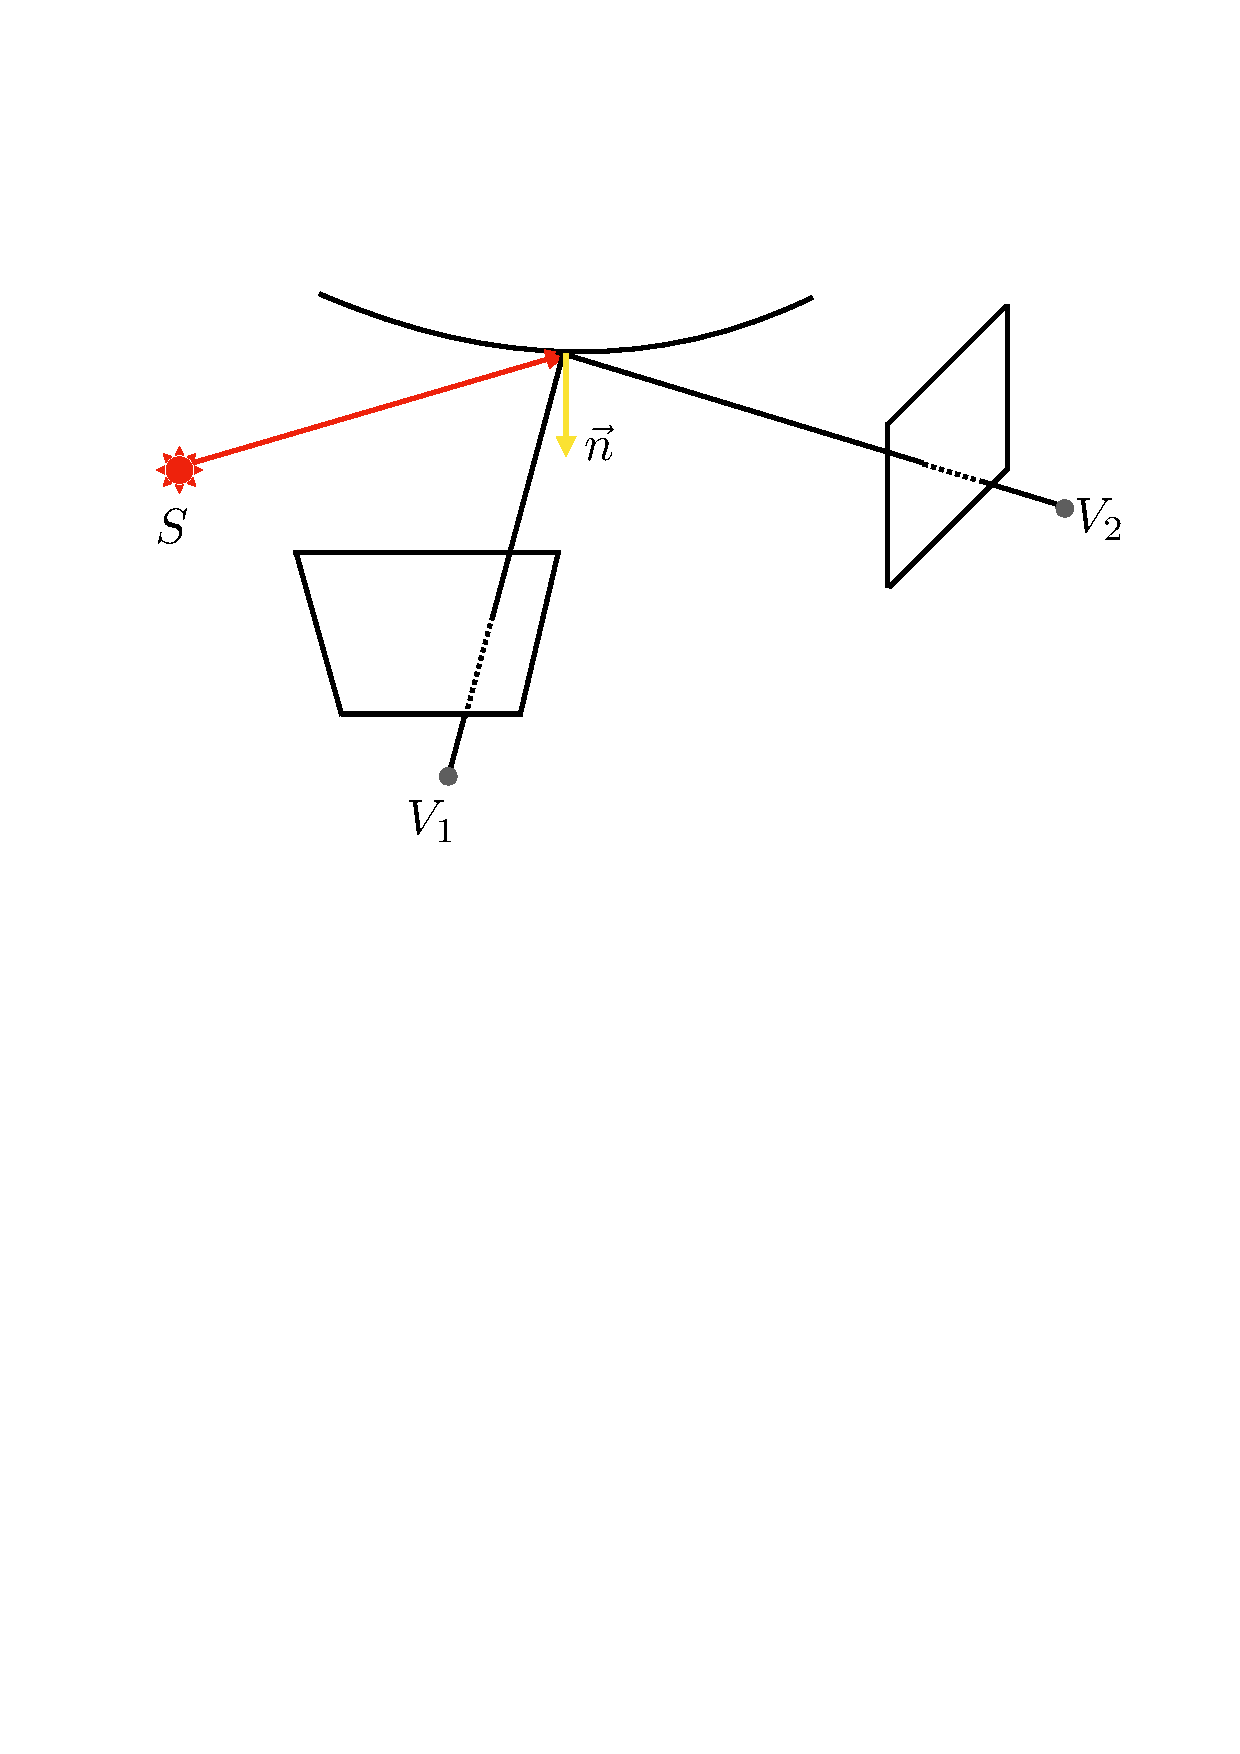
\includegraphics[width=0.22\textwidth]{mapping/mvs_spec/mvs_spec}&
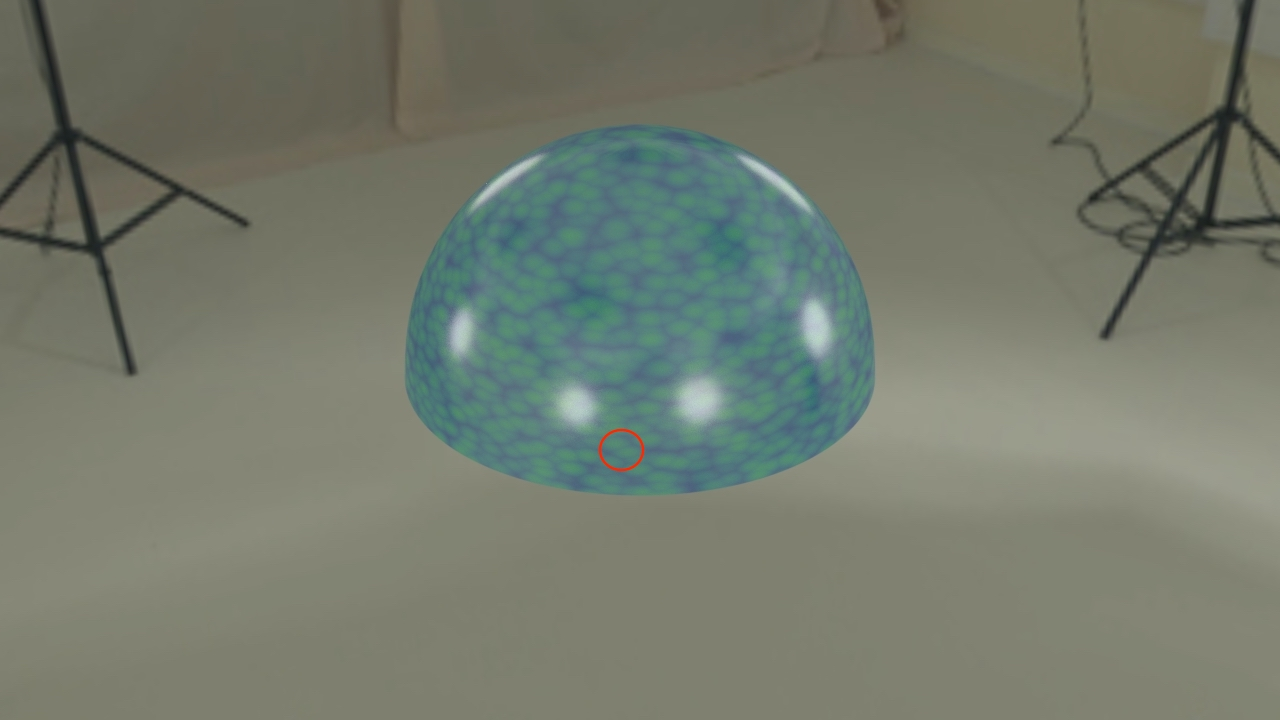
\includegraphics[width=0.22\textwidth]{mapping/mvs_spec/mvs_spec_01}&
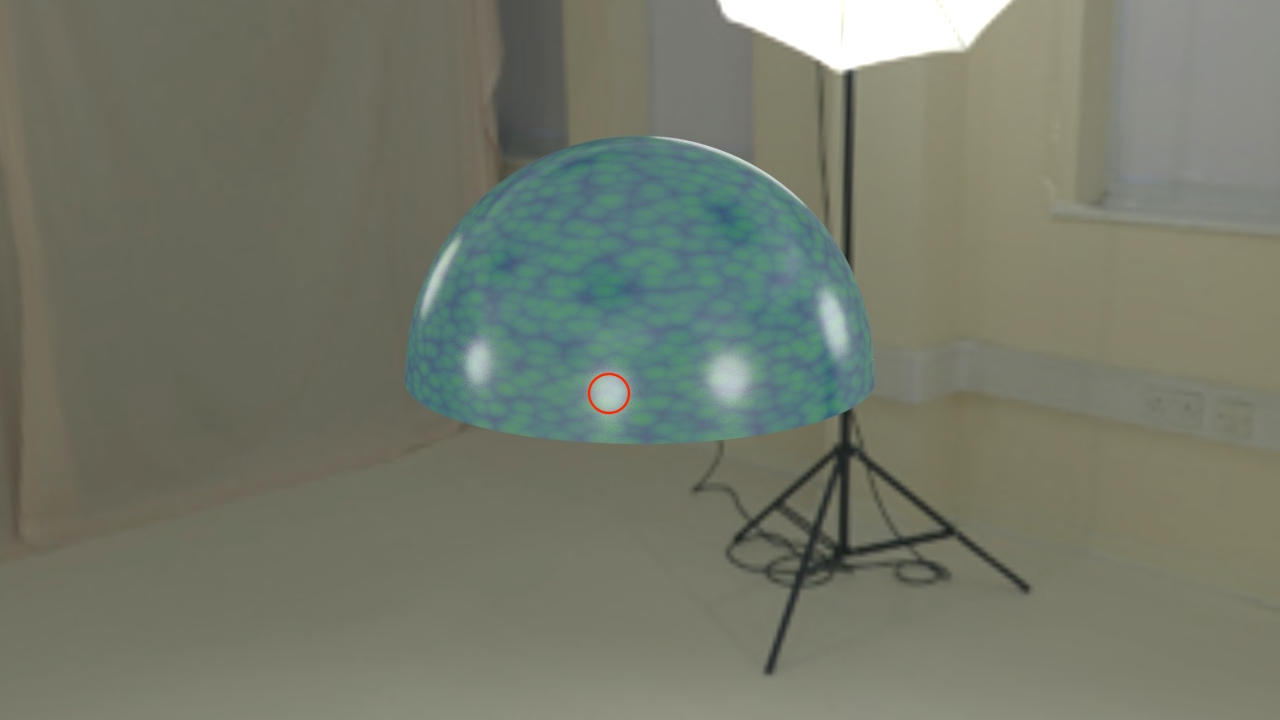
\includegraphics[width=0.22\textwidth]{mapping/mvs_spec/mvs_spec_00}\\
% (a). Image formation & (b) $V_1$ & (c) $V_2$\\
\end{tabular}
\end{figure}
\end{exampleblock}

\begin{exampleblock}{2. EPS and GSL fails on highly specular surfaces, and a blurred specular area leads to worse results.}
\begin{figure}
\begin{tabular}{ccc}
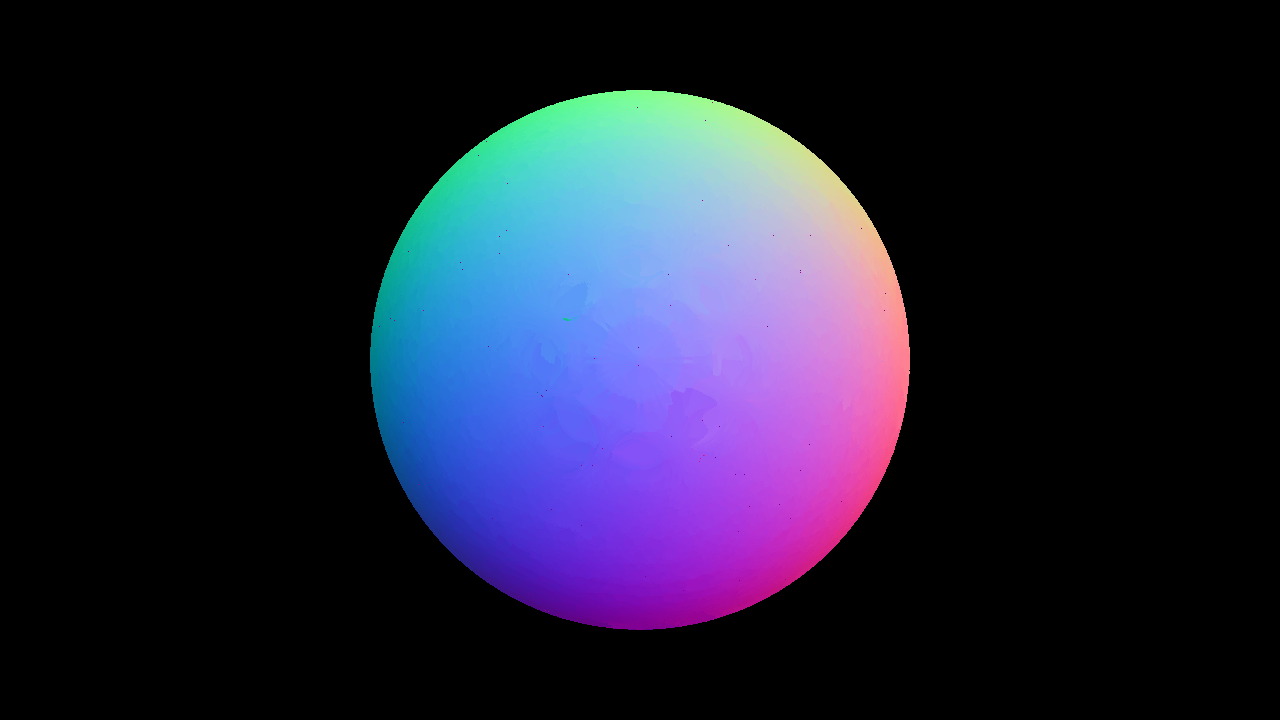
\includegraphics[width=0.15\textwidth]{mapping/ps_spec_rough/0802_normal}&
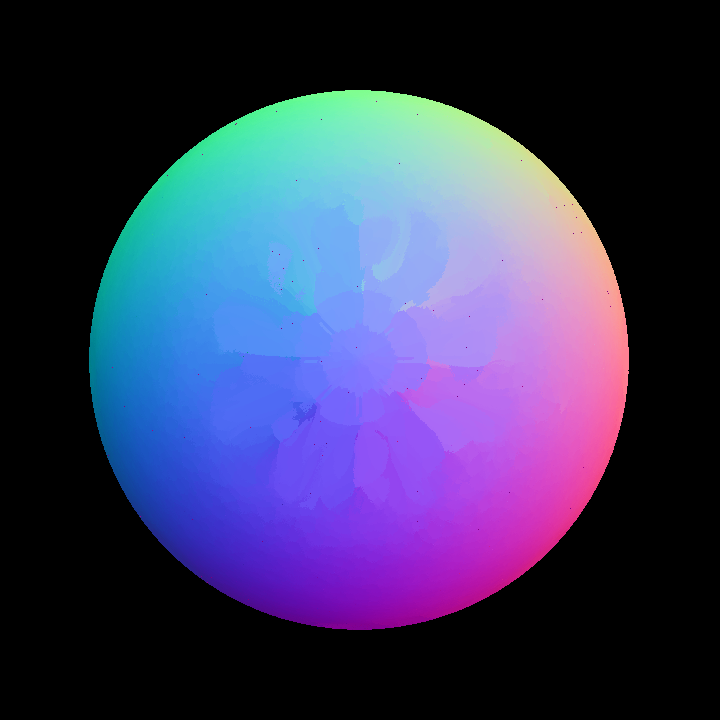
\includegraphics[width=0.15\textwidth]{mapping/ps_spec_rough/0805_normal}&
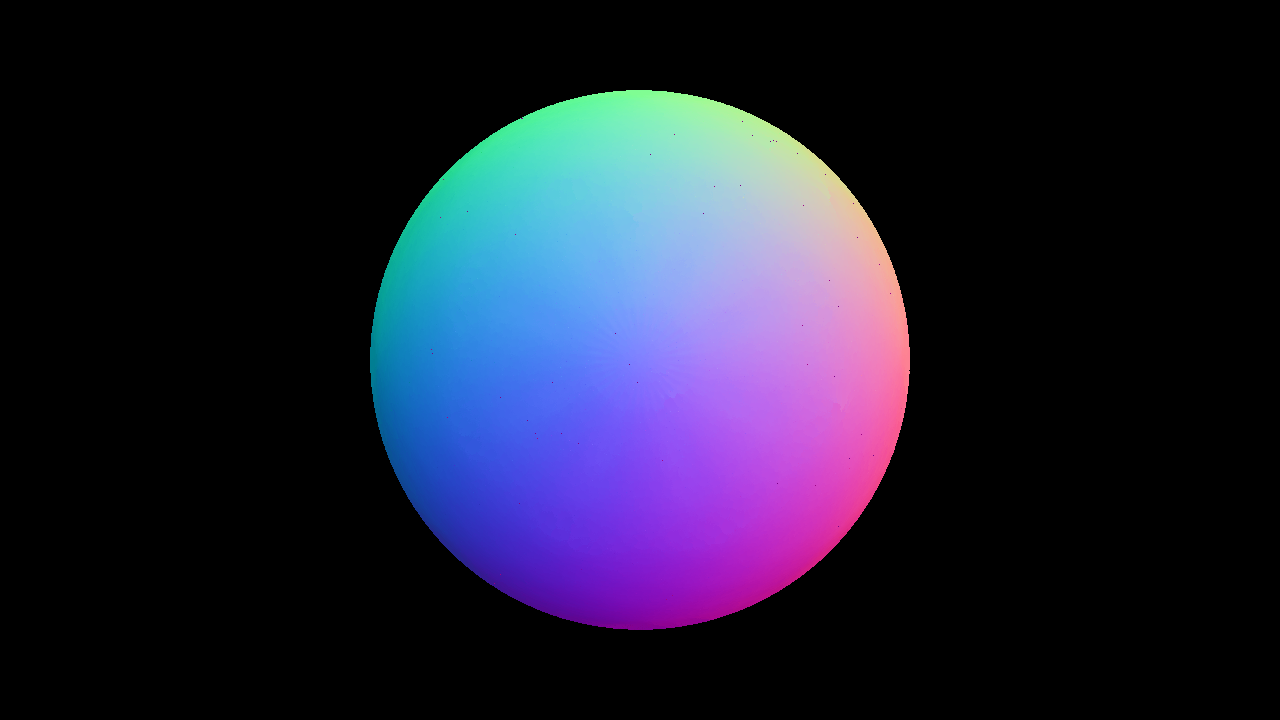
\includegraphics[width=0.15\textwidth]{mapping/ps_spec_rough/0808_normal}\\
(a). rough: 0.2 & (b). rough: 0.5 & (c). rough: 0.8
\end{tabular}
\end{figure}
\end{exampleblock}

\end{frame}

%------------------------------------------------
% \begin{frame}{Mapping: notable findings 1}

% \begin{figure}[!htbp]
% \begin{tabular}{cc}
% \includegraphics[width=0.22\textwidth]{mapping/pairwise/mvs_tex_spec}&
% 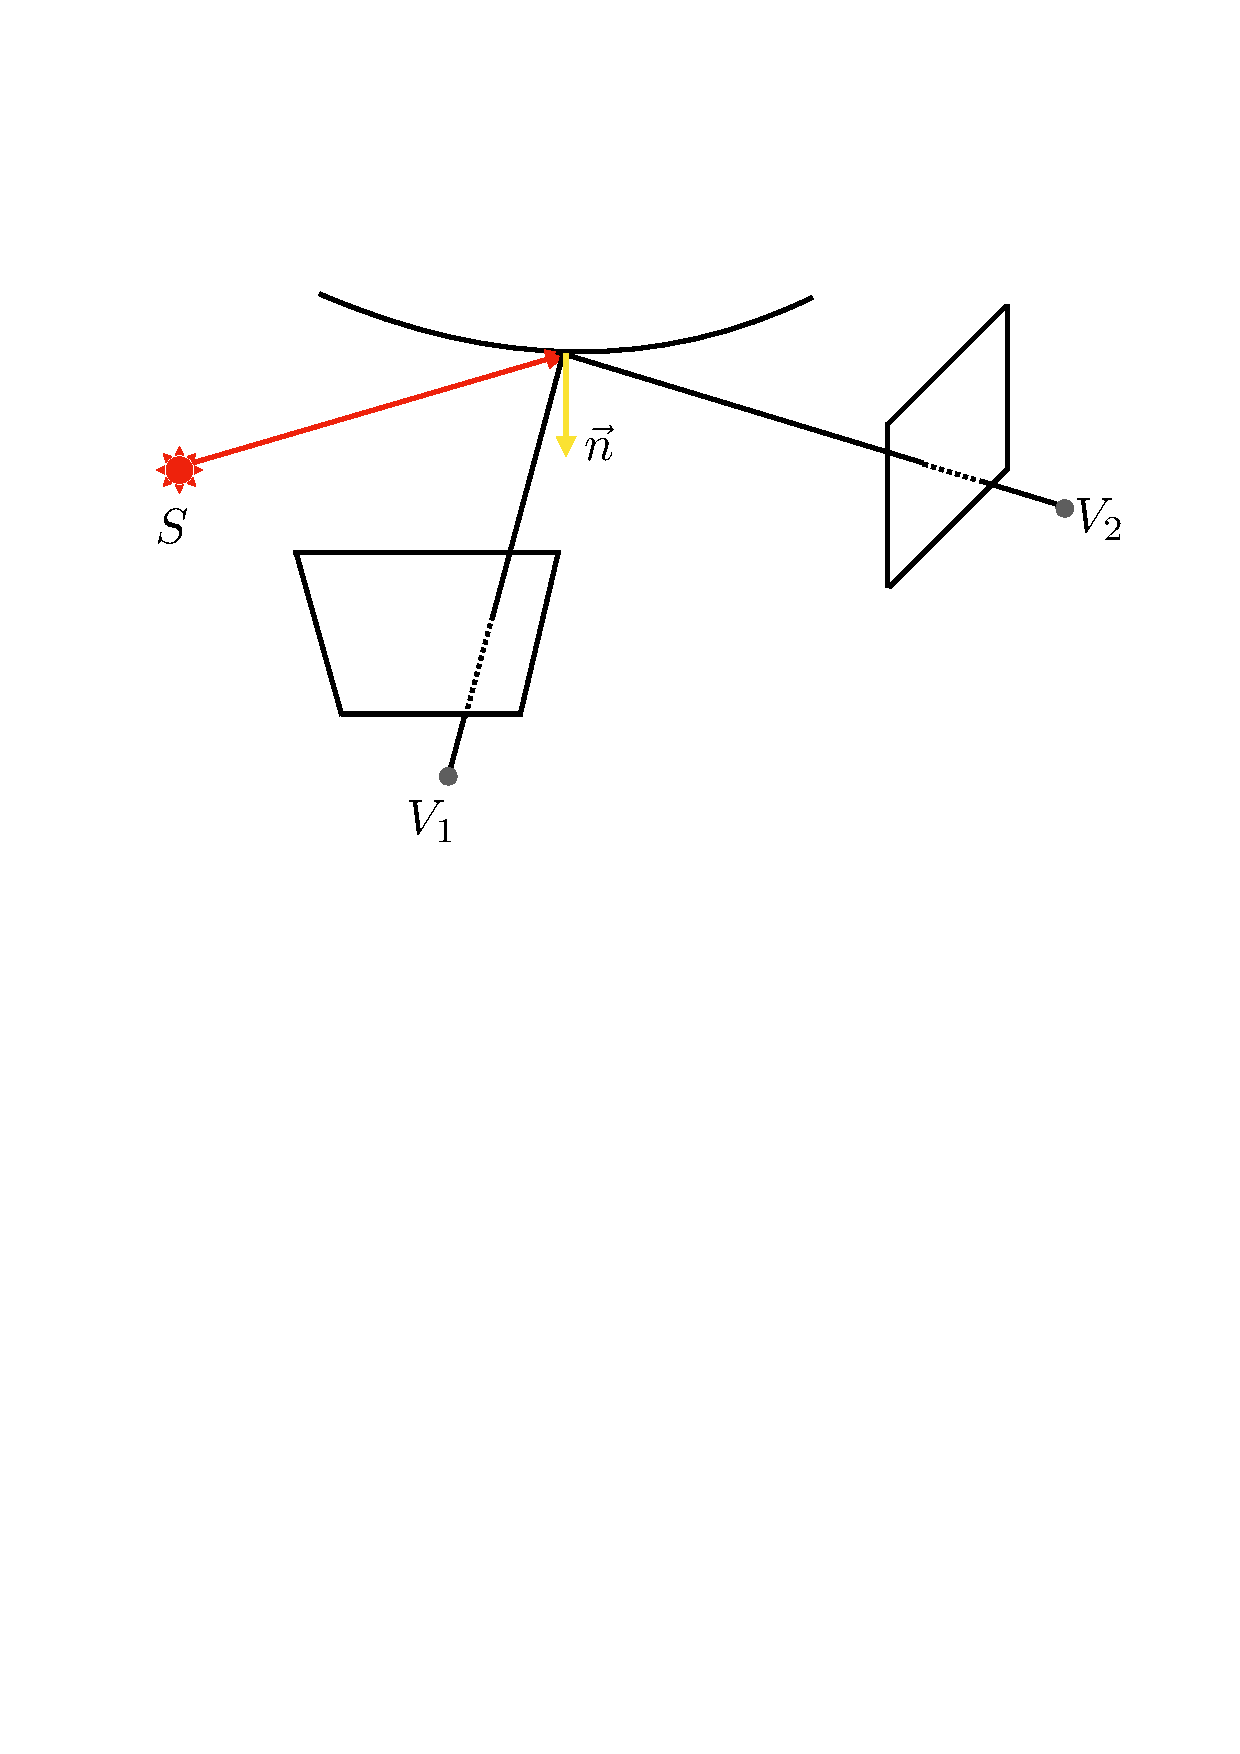
\includegraphics[width=0.22\textwidth]{mapping/mvs_spec/mvs_spec}\\
% (a). Algo. performance & (b) Image formation\\
% 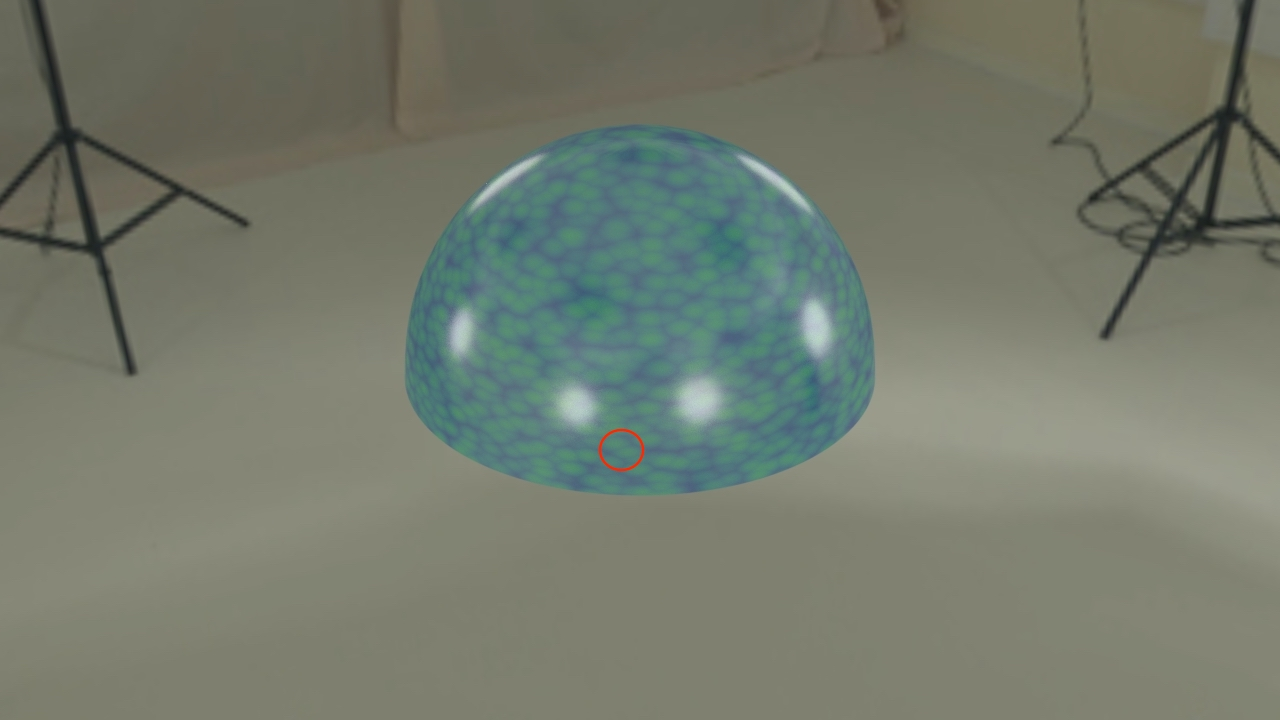
\includegraphics[width=0.22\textwidth]{mapping/mvs_spec/mvs_spec_01}&
% 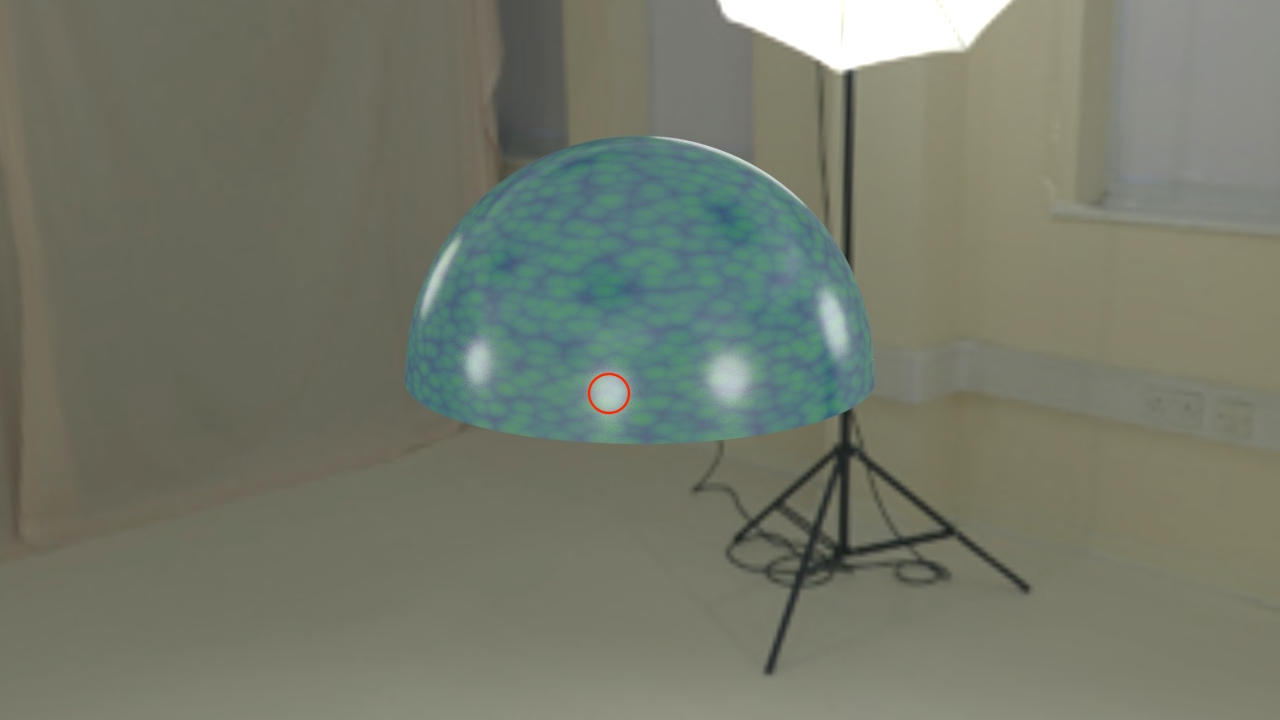
\includegraphics[width=0.22\textwidth]{mapping/mvs_spec/mvs_spec_00}\\
% (c) $V_1$ & (d) $V_2$\\
% \end{tabular}
% \caption{(a) shows the algorithm performance w.r.t. texture and specularity. (b) shows the reflection of light off a specular surface. $V_1$ received the diffuse component while $V_2$ receives the specular component. (c), (d) shows the images observed from these two views. The specular area (red circle) observed in $V_2$ is visible in $V_1$.}
% \end{figure}

% \end{frame}

%------------------------------------------------
% \begin{frame}{Mapping: notable findings 2}

% \begin{figure}[!htbp]
% \centering
% \begin{tabular}{c|ccc}
%   Image & Normal map & Height map & Angular error\\
%   \hline\\
%   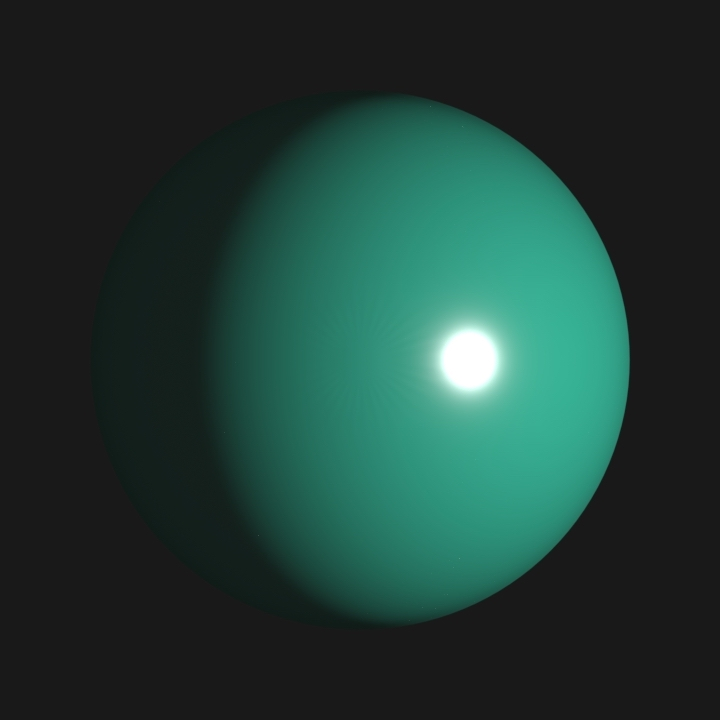
\includegraphics[width=0.12\textwidth]{mapping/ps_spec_rough/0802_0001}&
%   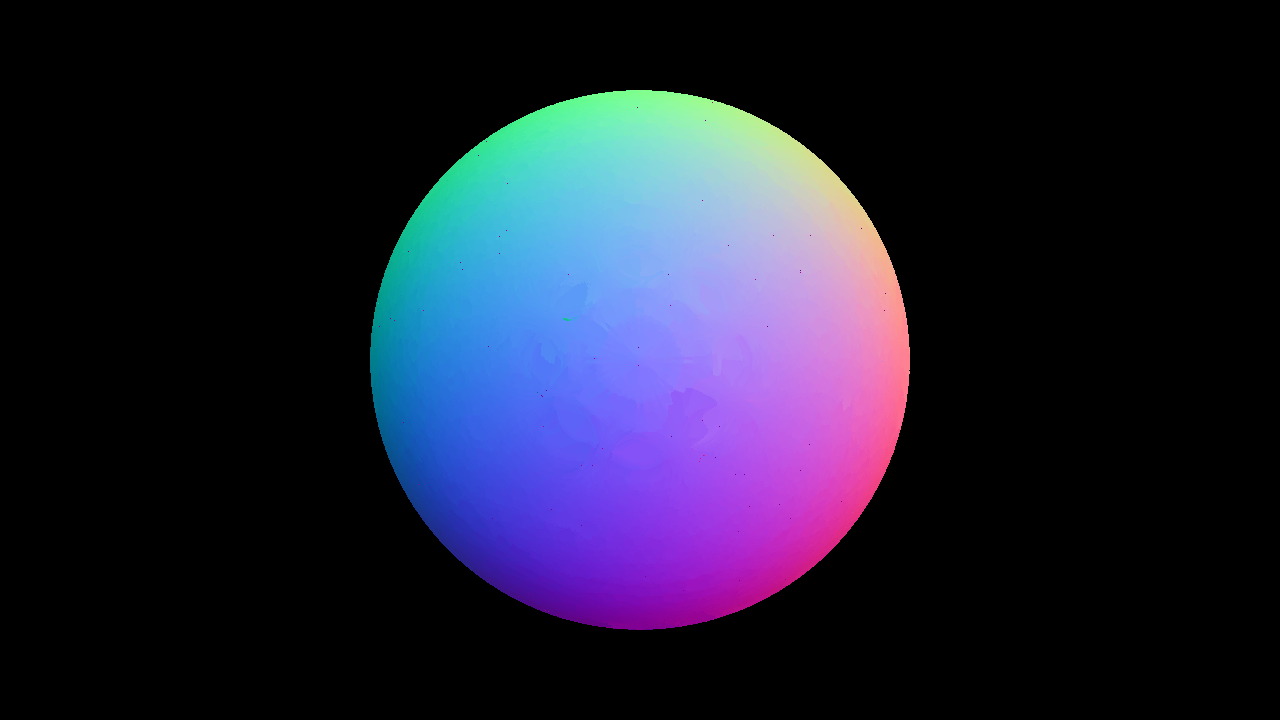
\includegraphics[width=0.12\textwidth]{mapping/ps_spec_rough/0802_normal}&
%   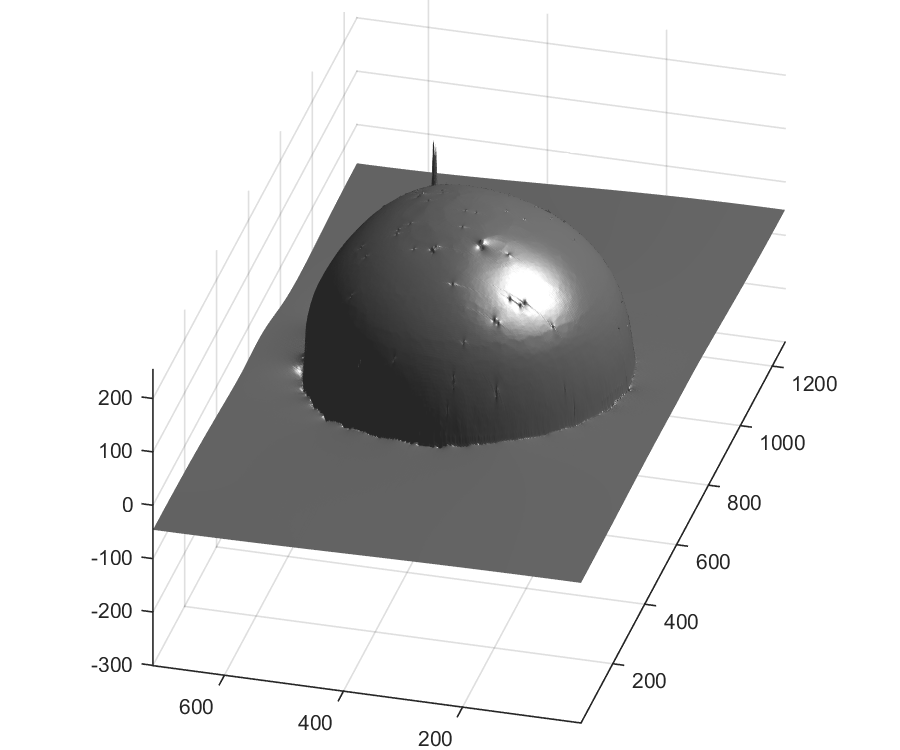
\includegraphics[width=0.15\textwidth]{images/0802_dmap}&
%   \includegraphics[width=0.05\textwidth]{mapping/ps_spec_rough/0802_ang_error}\\
%   & (a). rough: 0.2\\
%   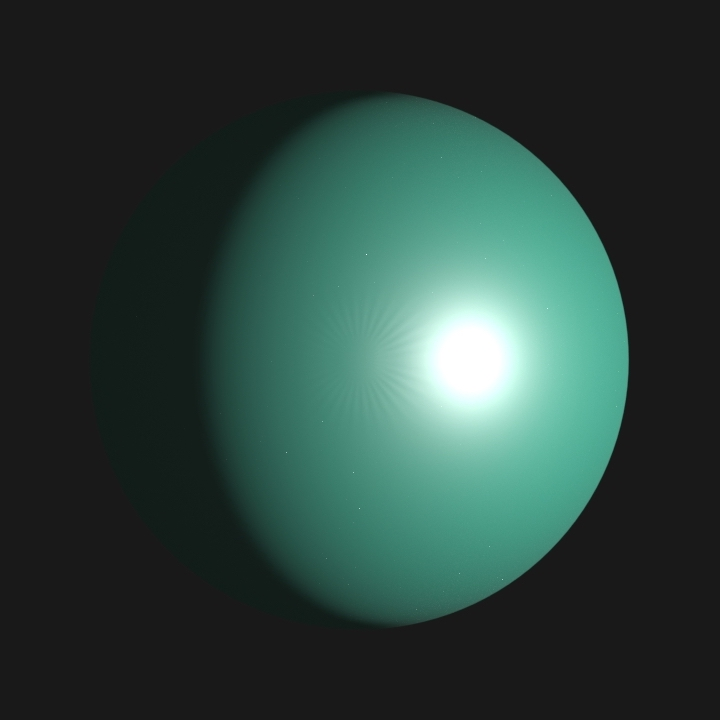
\includegraphics[width=0.12\textwidth]{mapping/ps_spec_rough/0805_0001}&
%   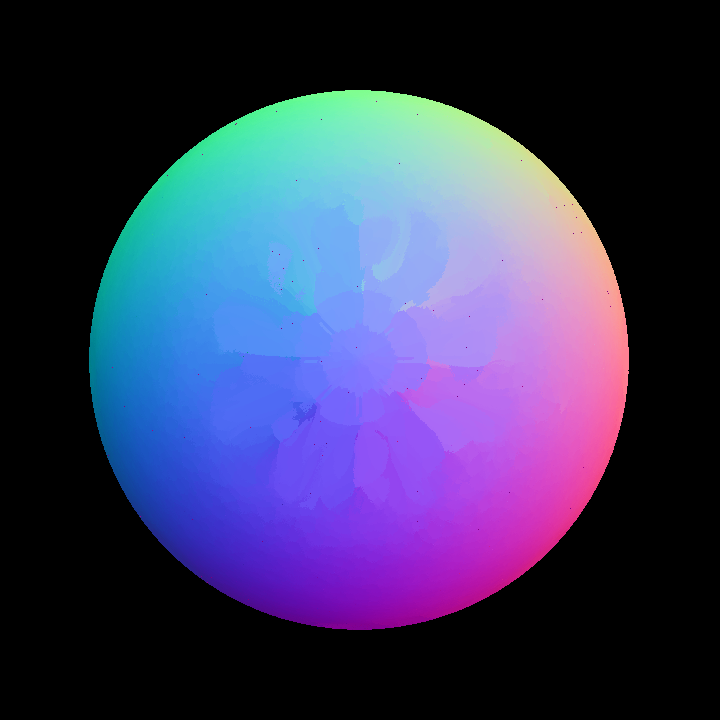
\includegraphics[width=0.12\textwidth]{mapping/ps_spec_rough/0805_normal}&
%   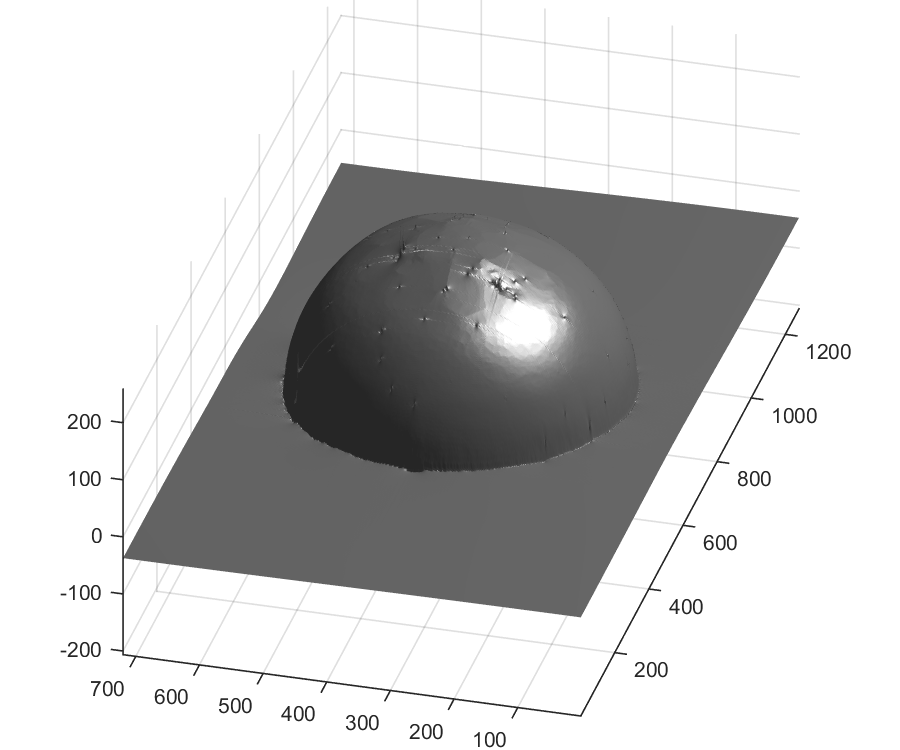
\includegraphics[width=0.15\textwidth]{images/0805_dmap}&
%   \includegraphics[width=0.05\textwidth]{mapping/ps_spec_rough/0805_ang_error}\\
%   & (b). rough: 0.5\\
%   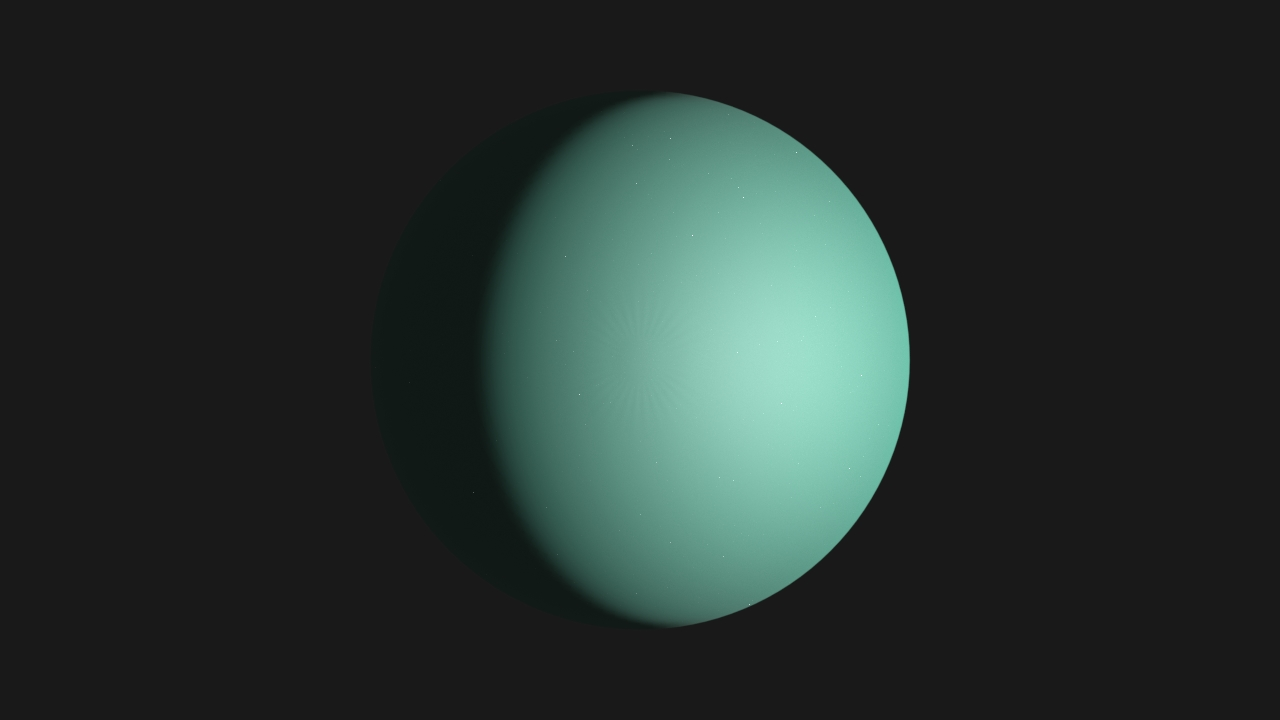
\includegraphics[width=0.12\textwidth]{mapping/ps_spec_rough/0808_0001}&
%   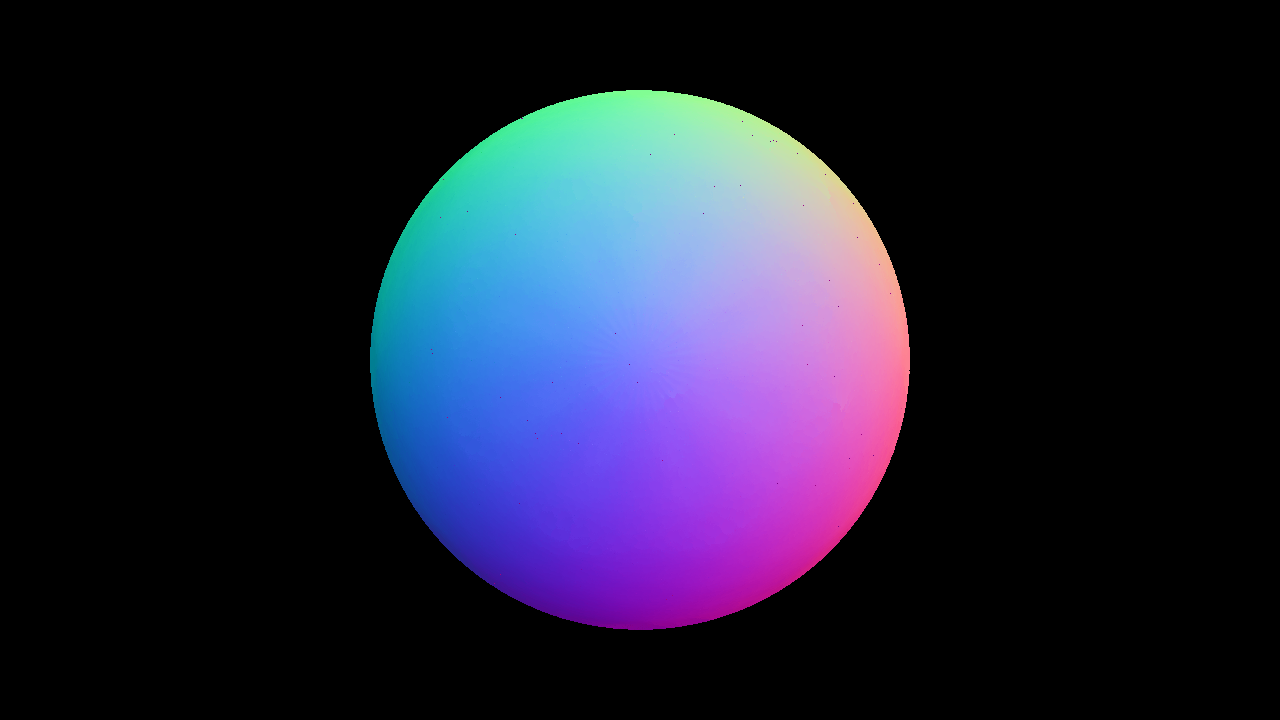
\includegraphics[width=0.12\textwidth]{mapping/ps_spec_rough/0808_normal}&
%   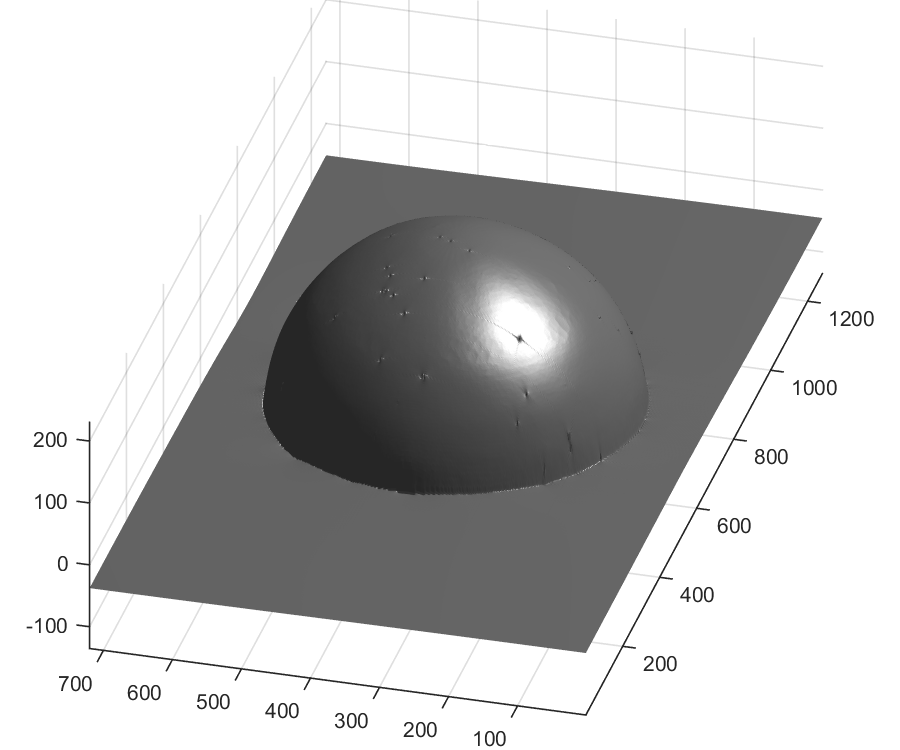
\includegraphics[width=0.15\textwidth]{images/0808_dmap}&
%   \includegraphics[width=0.05\textwidth]{mapping/ps_spec_rough/0808_ang_error}\\
%   & (c). rough: 0.8\\
% \end{tabular}
% \caption{The effect of roughness on PS. Albedo is set as 0.8, and specular is set as 0.8. (b) demonstrates that a medium level roughness would lead to worse normal estimation since it blurs the specular lobe.}
% \end{figure}

% \end{frame}

%------------------------------------------------
% \begin{frame}{Mapping: notable findings 3}

% \begin{figure}[!htbp]
% \centering
% \begin{tabular}{ccc}
% 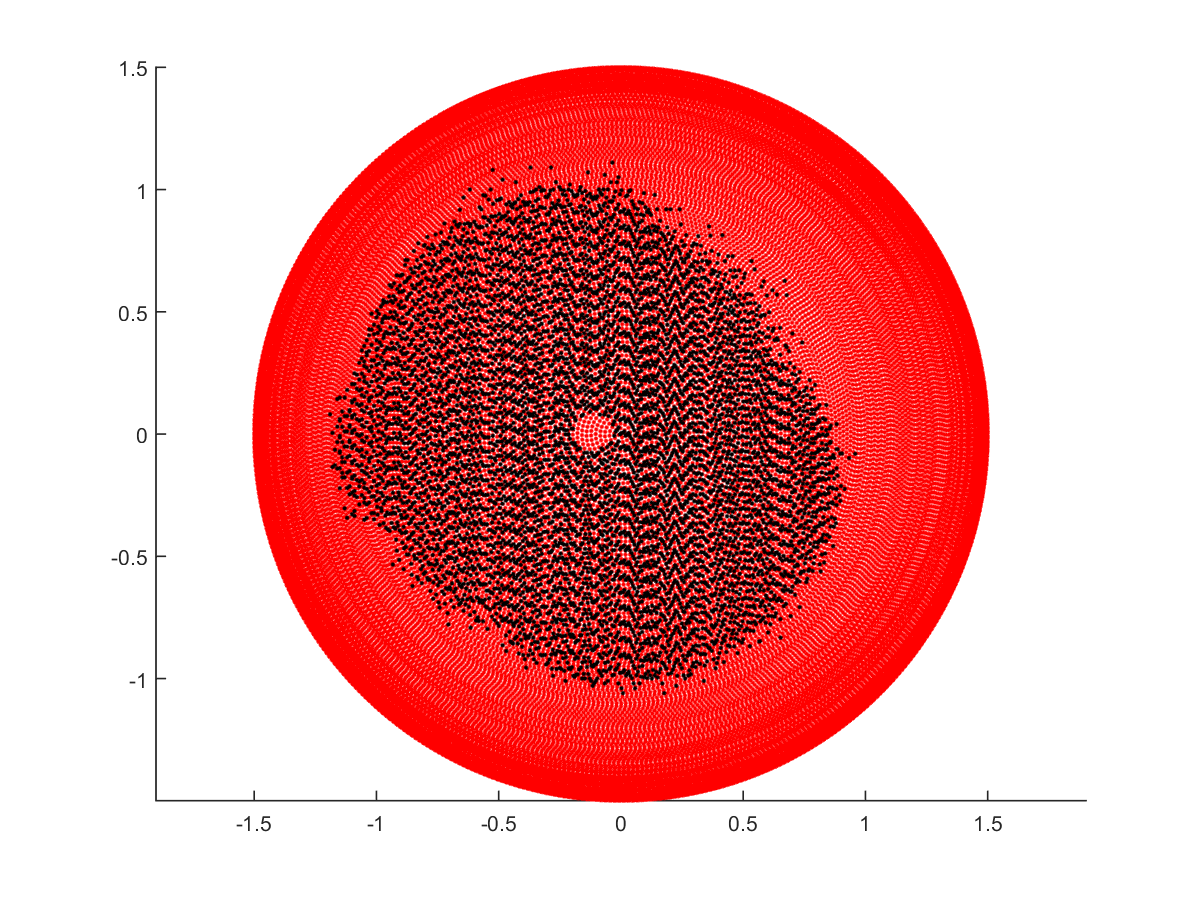
\includegraphics[width=0.25\textwidth]{trash/mapping/sl_spec_rough/sl_00050202}&
% 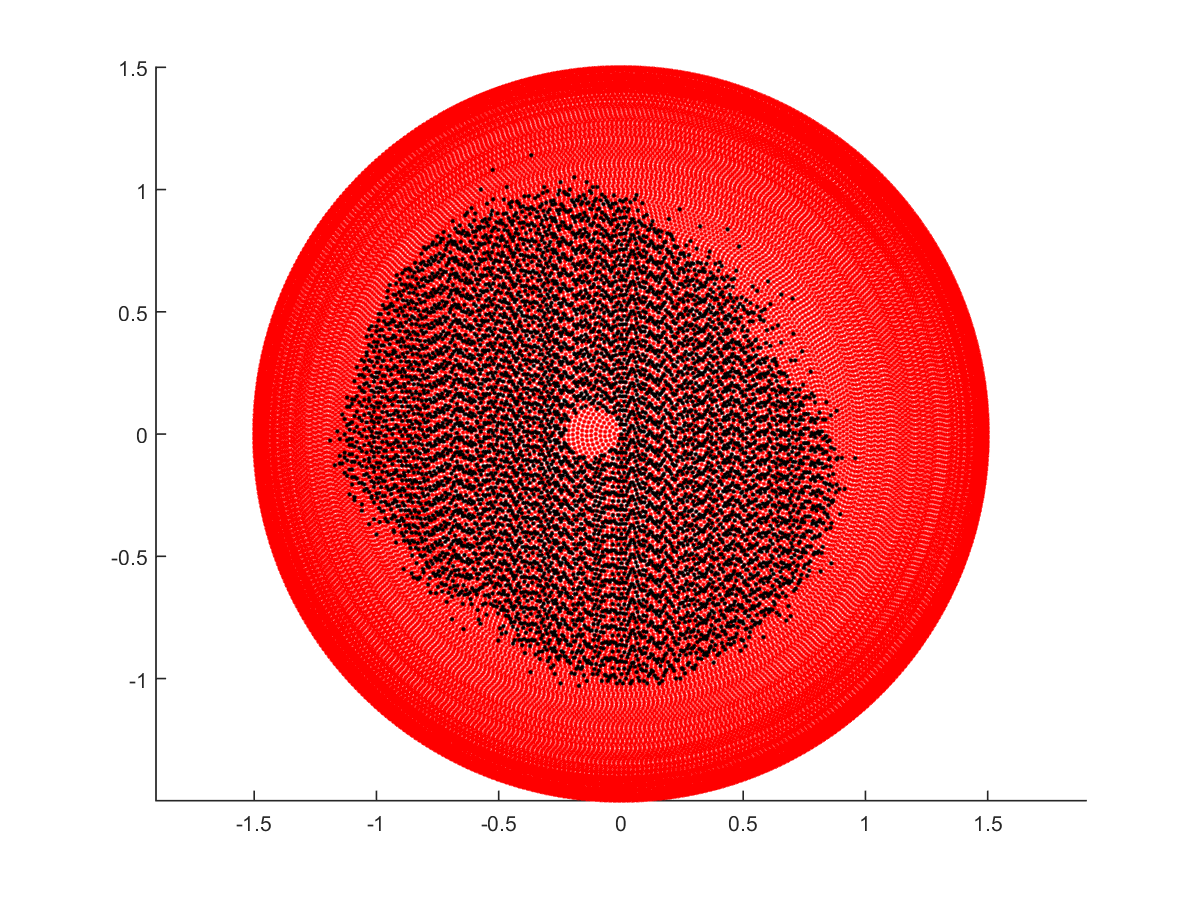
\includegraphics[width=0.25\textwidth]{trash/mapping/sl_spec_rough/sl_00050502}&
% 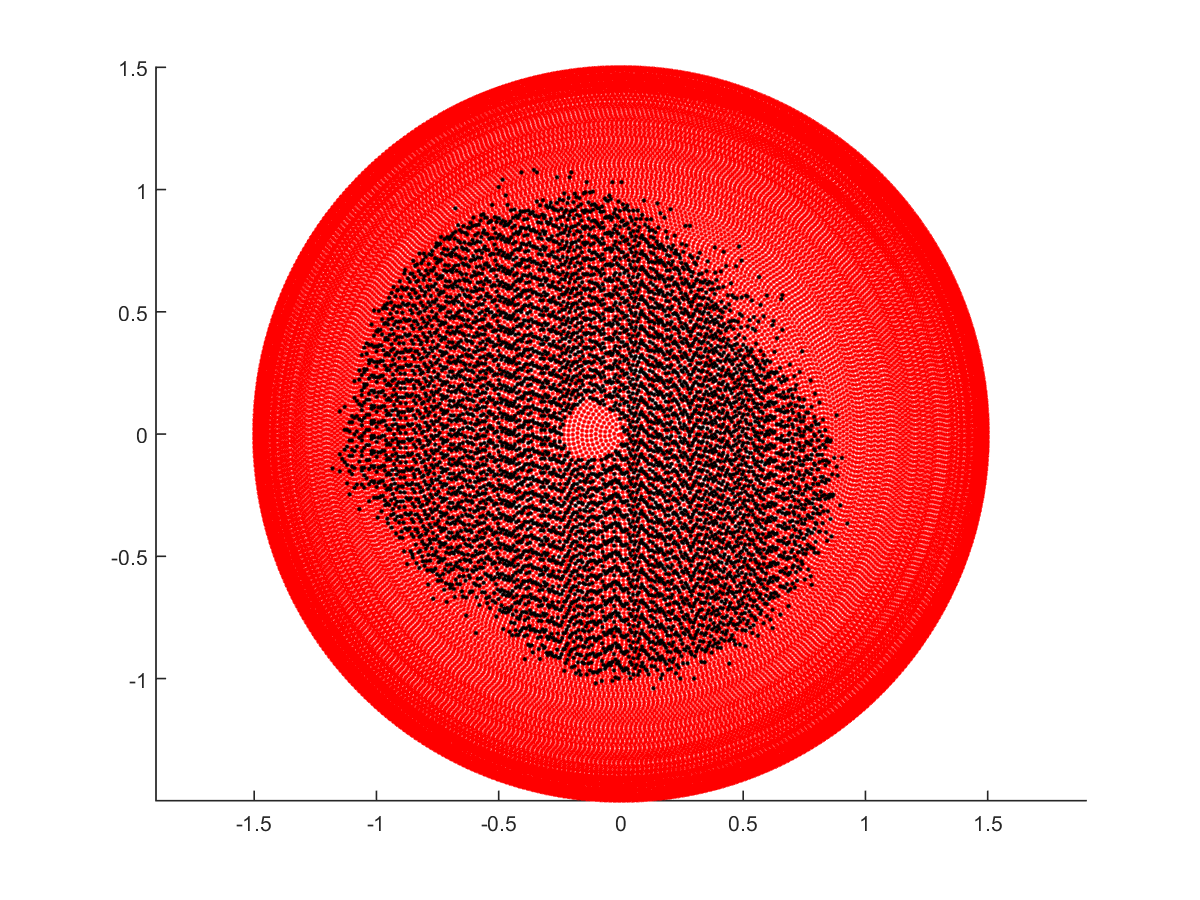
\includegraphics[width=0.25\textwidth]{trash/mapping/sl_spec_rough/sl_00050802}\\
% (a) specular: 0.2 & (b) specular: 0.5 & (c) specular: 0.8\\
% 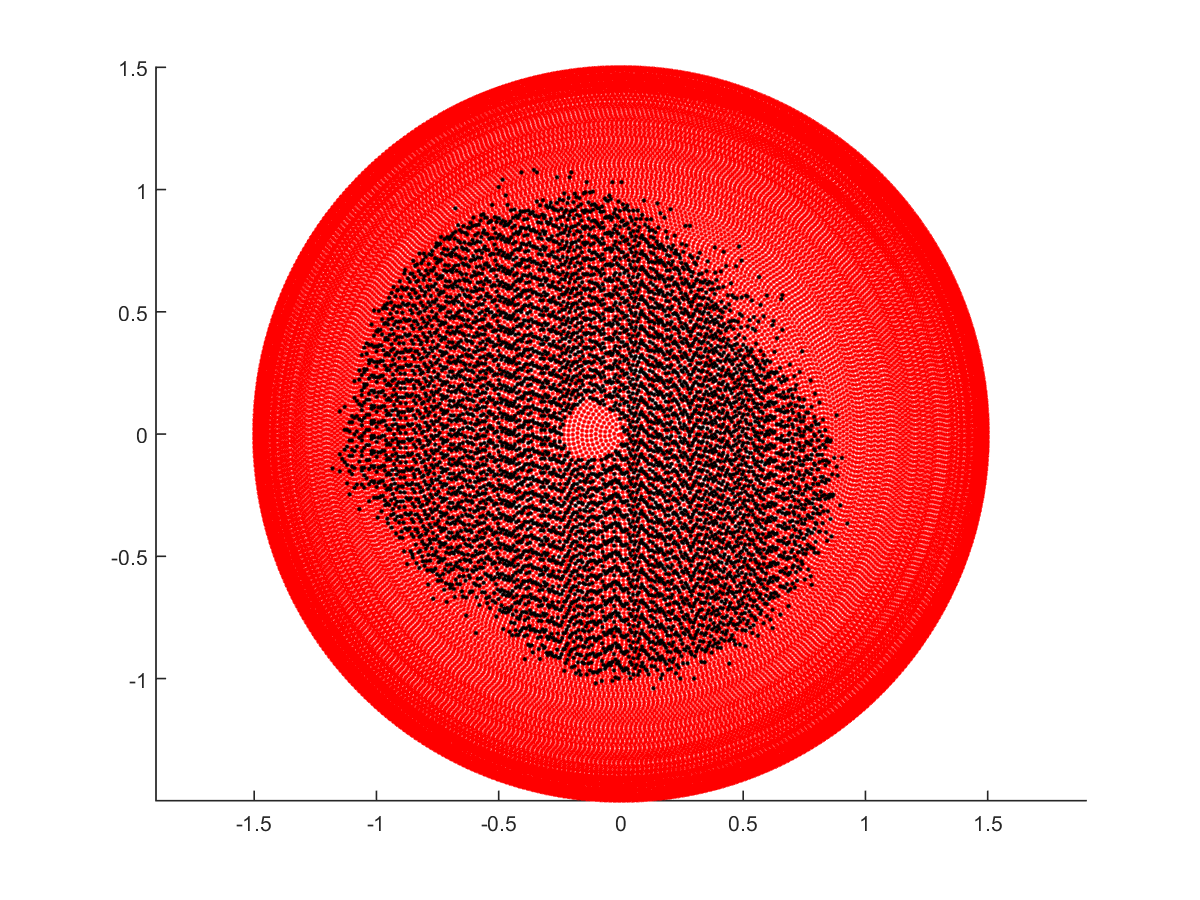
\includegraphics[width=0.25\textwidth]{trash/mapping/sl_spec_rough/sl_00050802}&
% 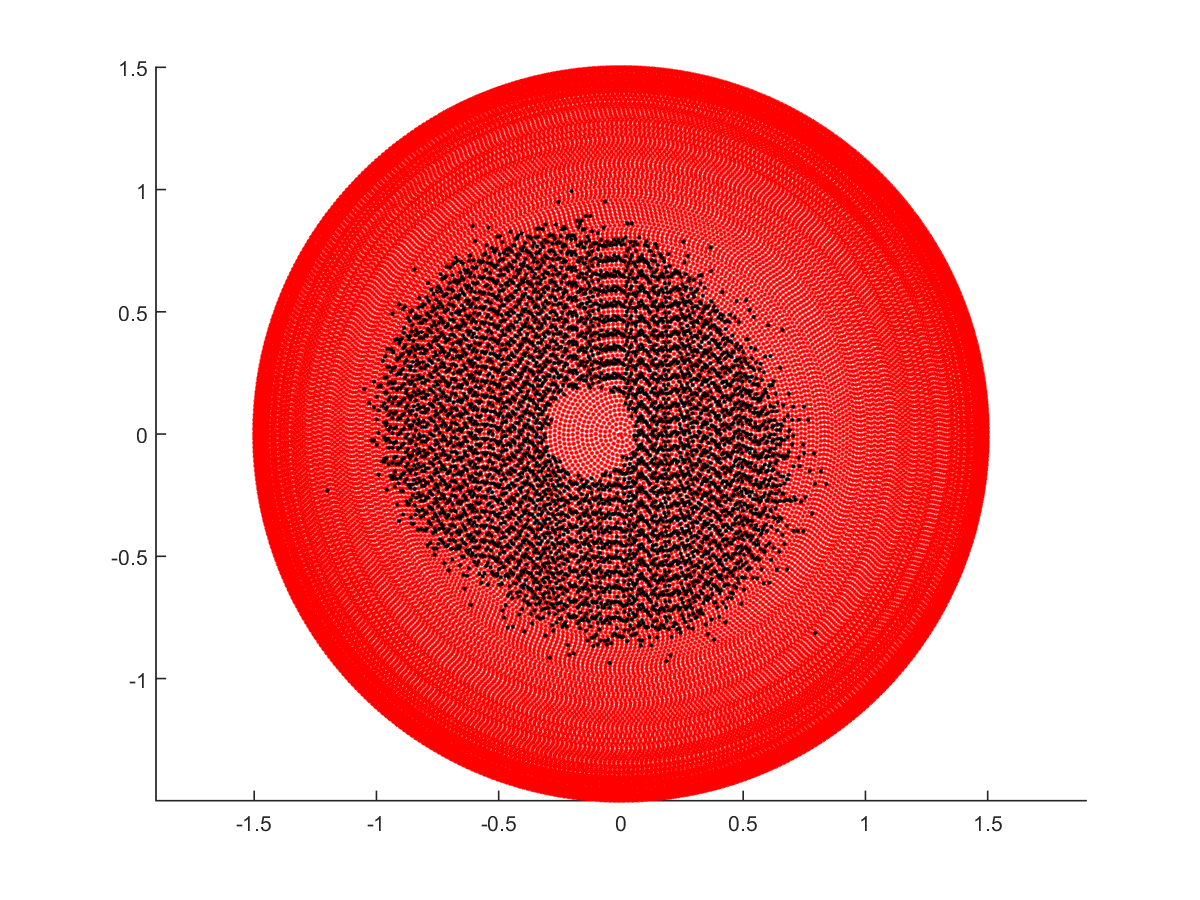
\includegraphics[width=0.25\textwidth]{trash/mapping/sl_spec_rough/sl_00050805}&
% 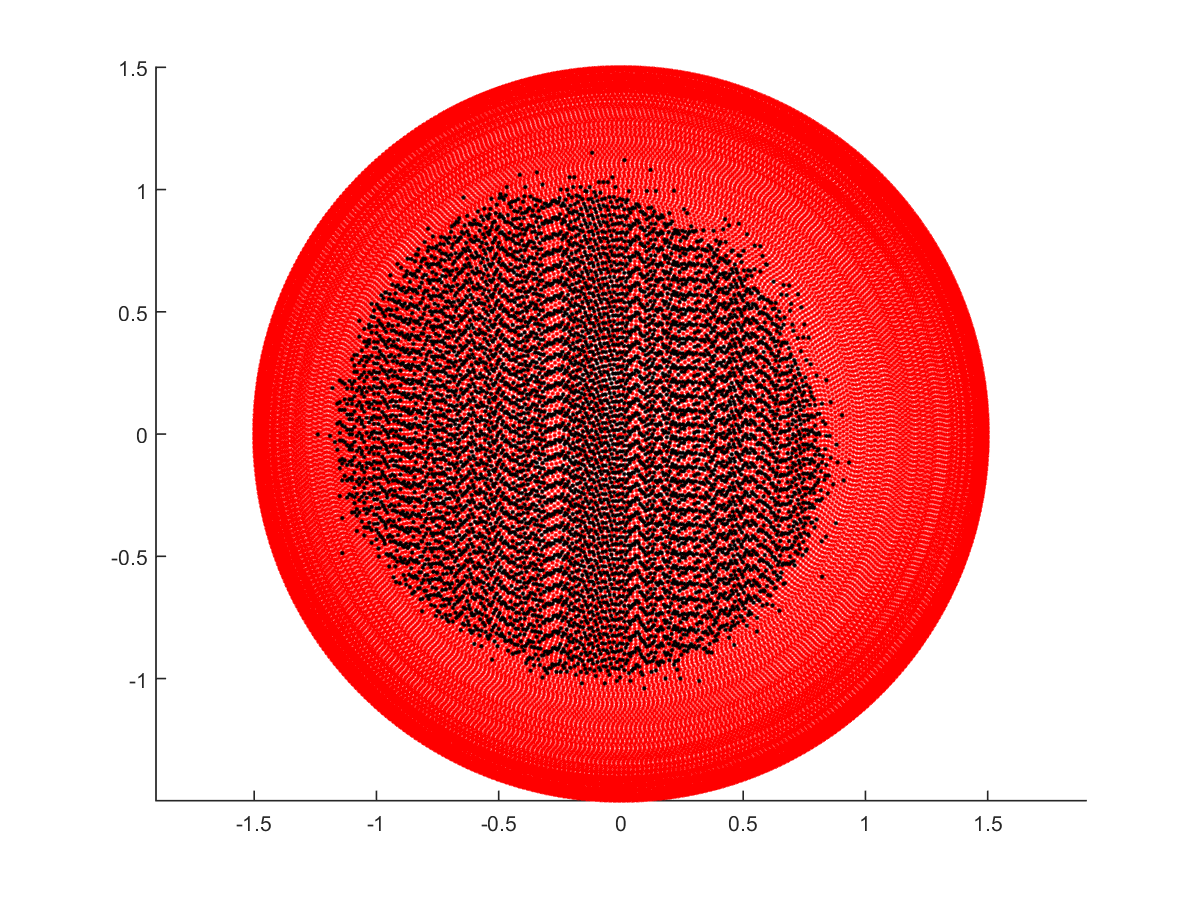
\includegraphics[width=0.25\textwidth]{trash/mapping/sl_spec_rough/sl_00050808}\\
% (d) roughness: 0.2 & (e) roughness: 0.5 & (f) roughness: 0.8\\
% \end{tabular}
% \caption{(a)-(c): the roughness is set as 0.2, and specular has a negative effect on completeness; (d)-(e): the specular is set as 0.8, roughness has a positive effect on completeness.}
% \end{figure}

% \end{frame}

%------------------------------------------------
\begin{frame}{Interpretation: dataset}

Objects meet the requirements of the four problem conditions.

\begin{figure}[!htbp]
\centering
\begin{tabular}{*{4}{c}} % p{1.5cm}
1 & 2 & 3 & 4\\
\midrule 
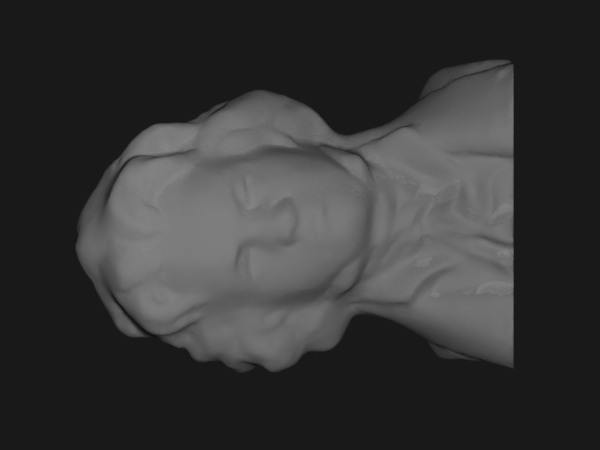
\includegraphics[width=0.15\textwidth]{interp/synth_data/bust} &
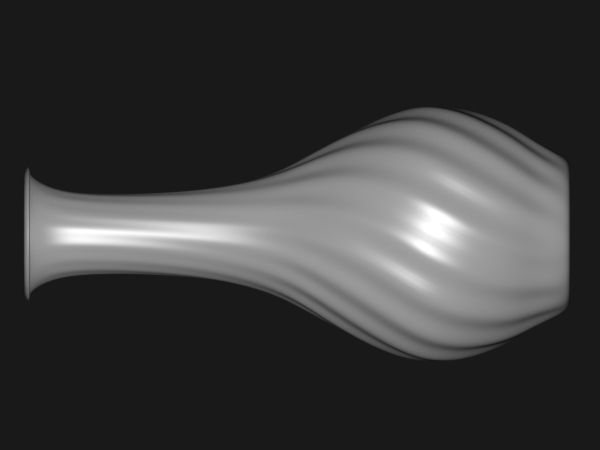
\includegraphics[width=0.15\textwidth]{interp/synth_data/vase0} &
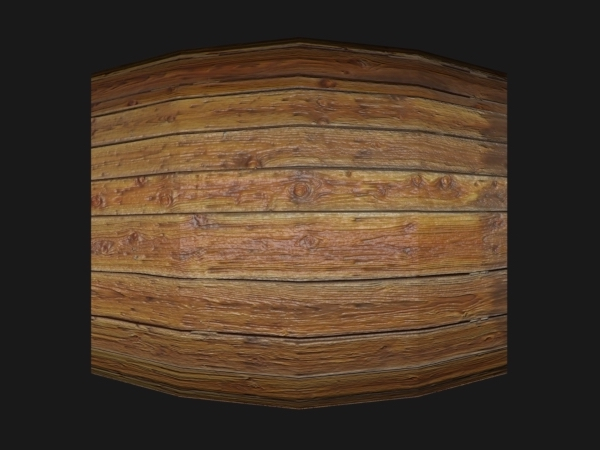
\includegraphics[width=0.15\textwidth]{interp/synth_data/barrel} &
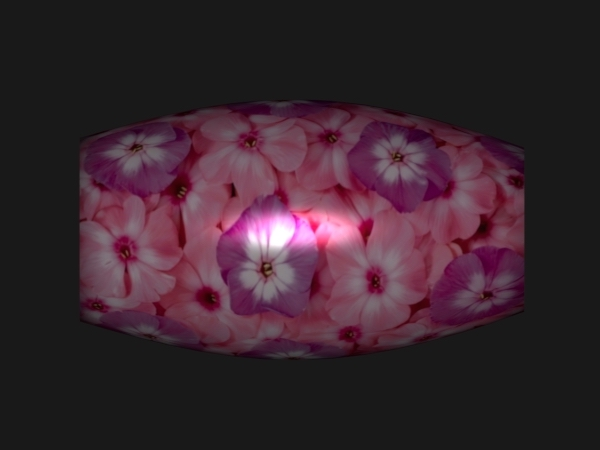
\includegraphics[width=0.15\textwidth]{interp/synth_data/vase1}\\
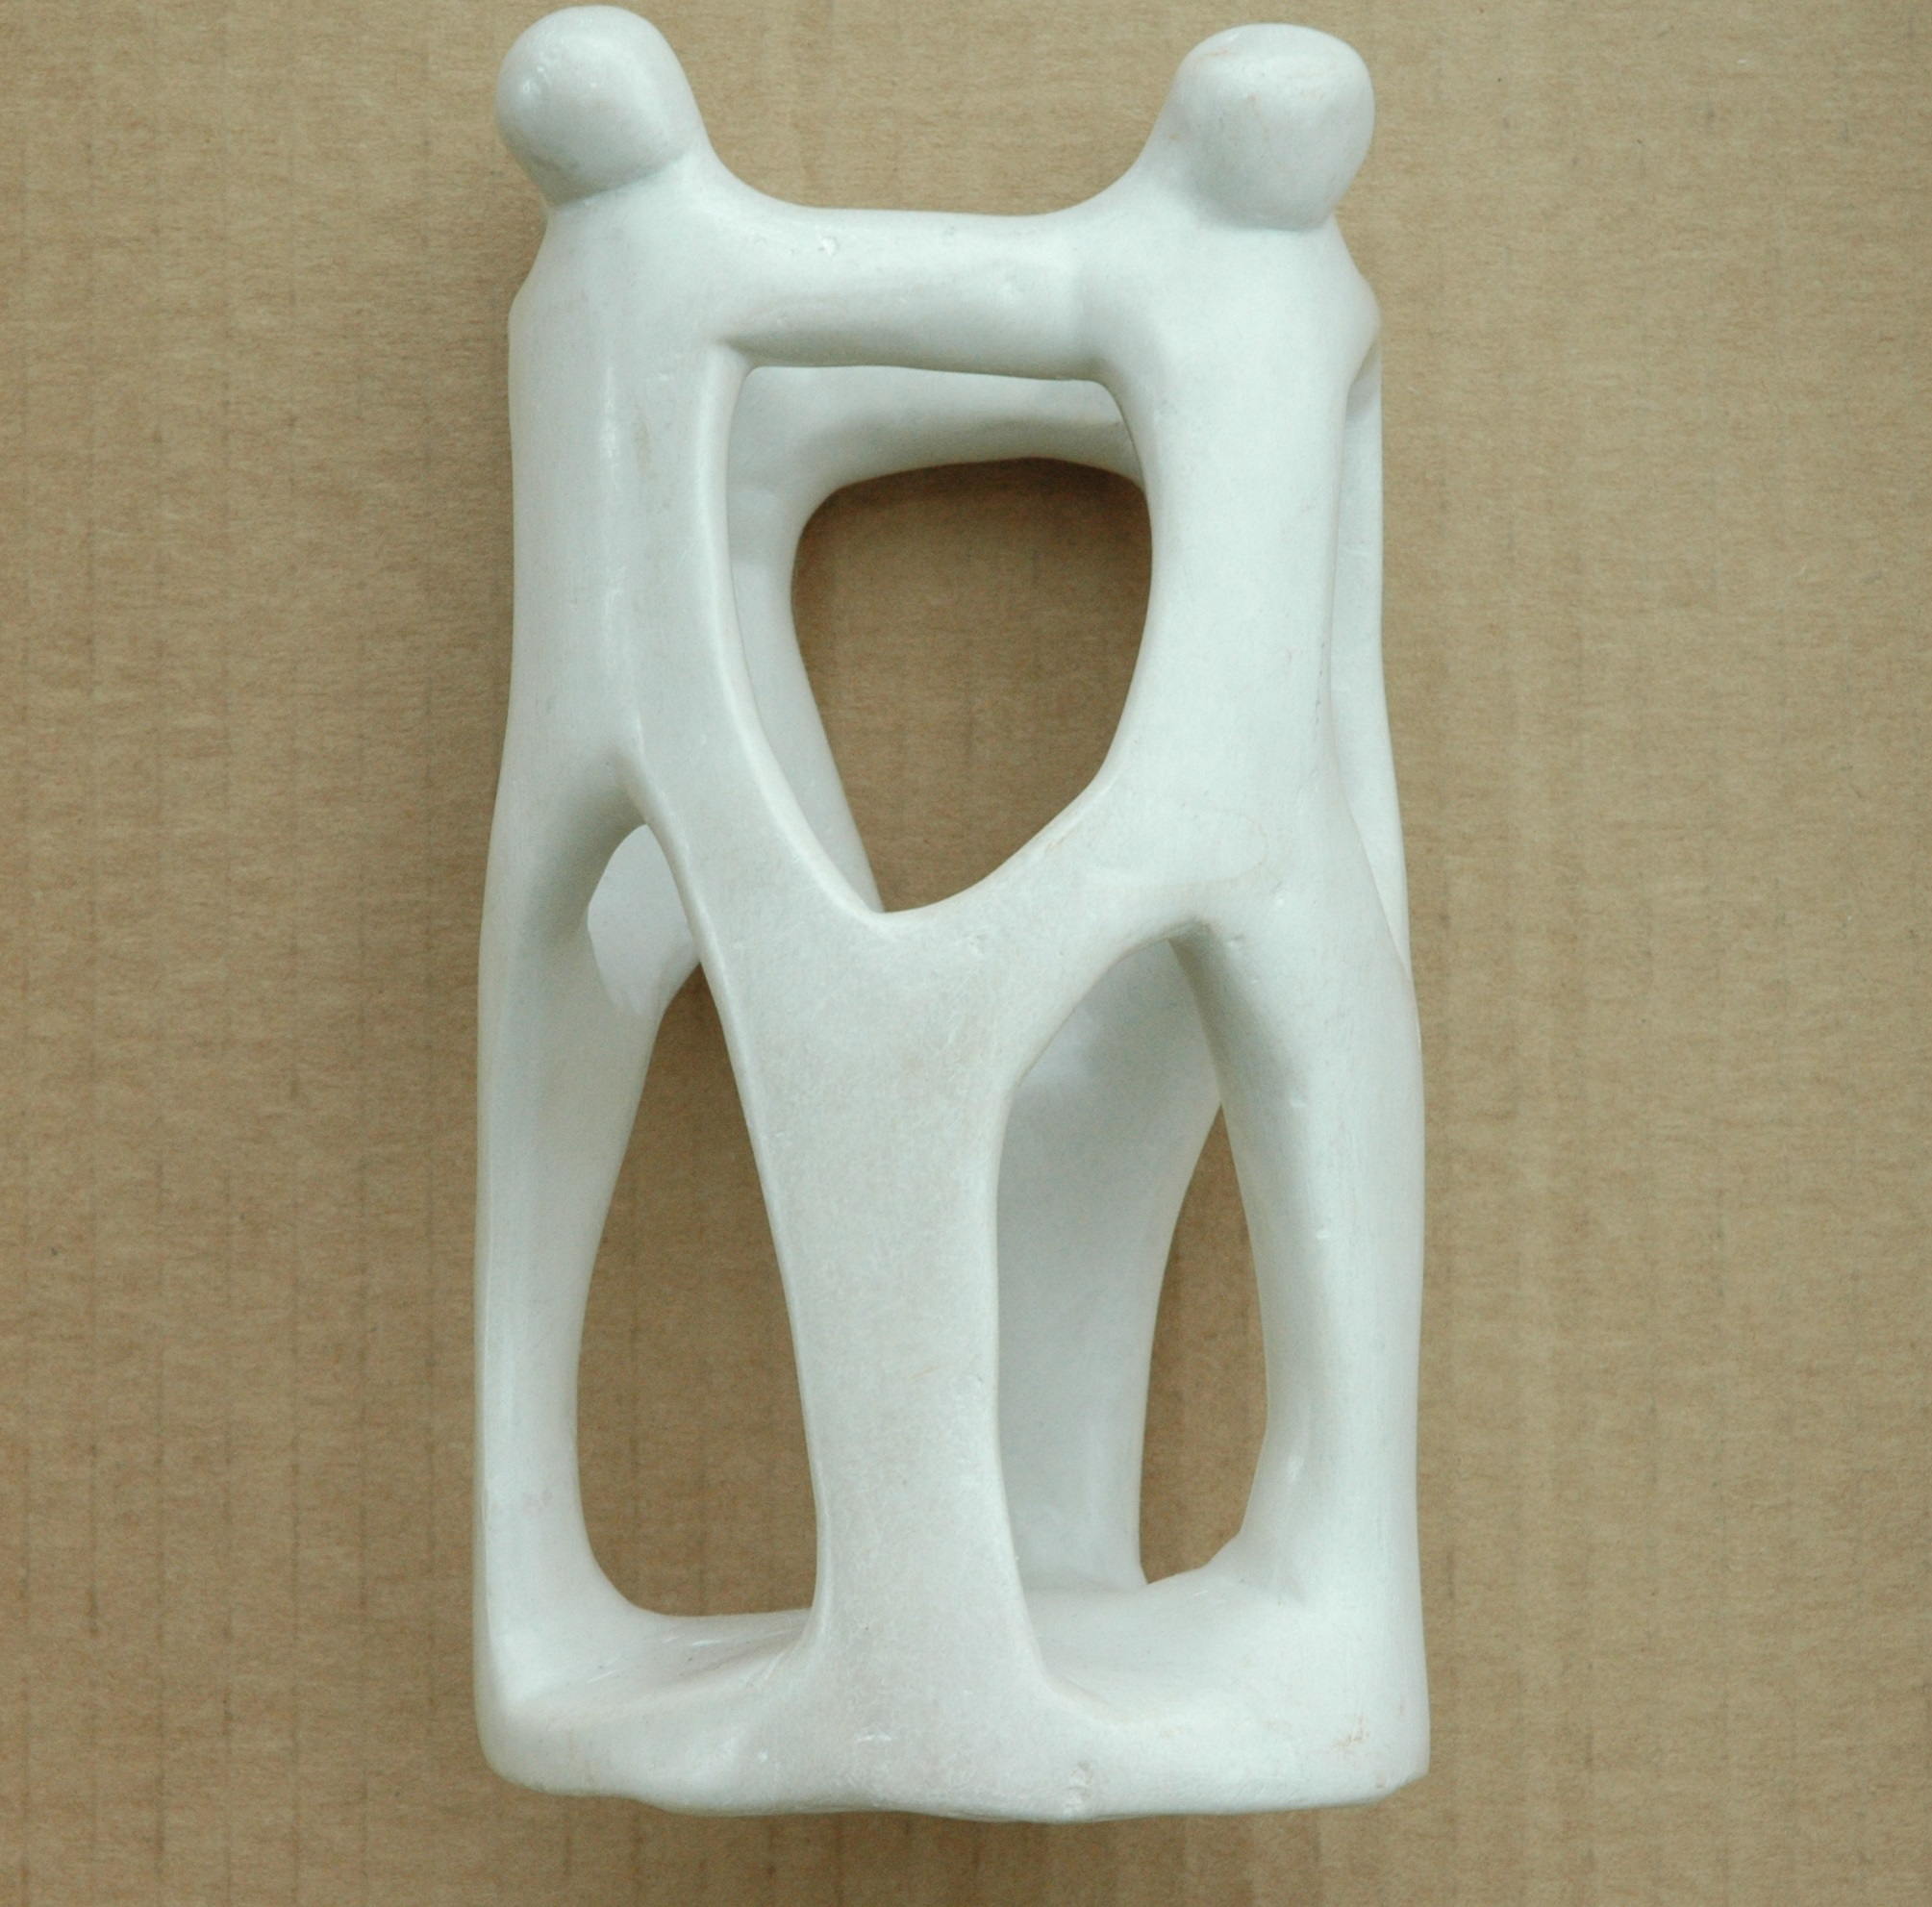
\includegraphics[width=0.15\textwidth]{interp/real_world_img/statue/statue} &
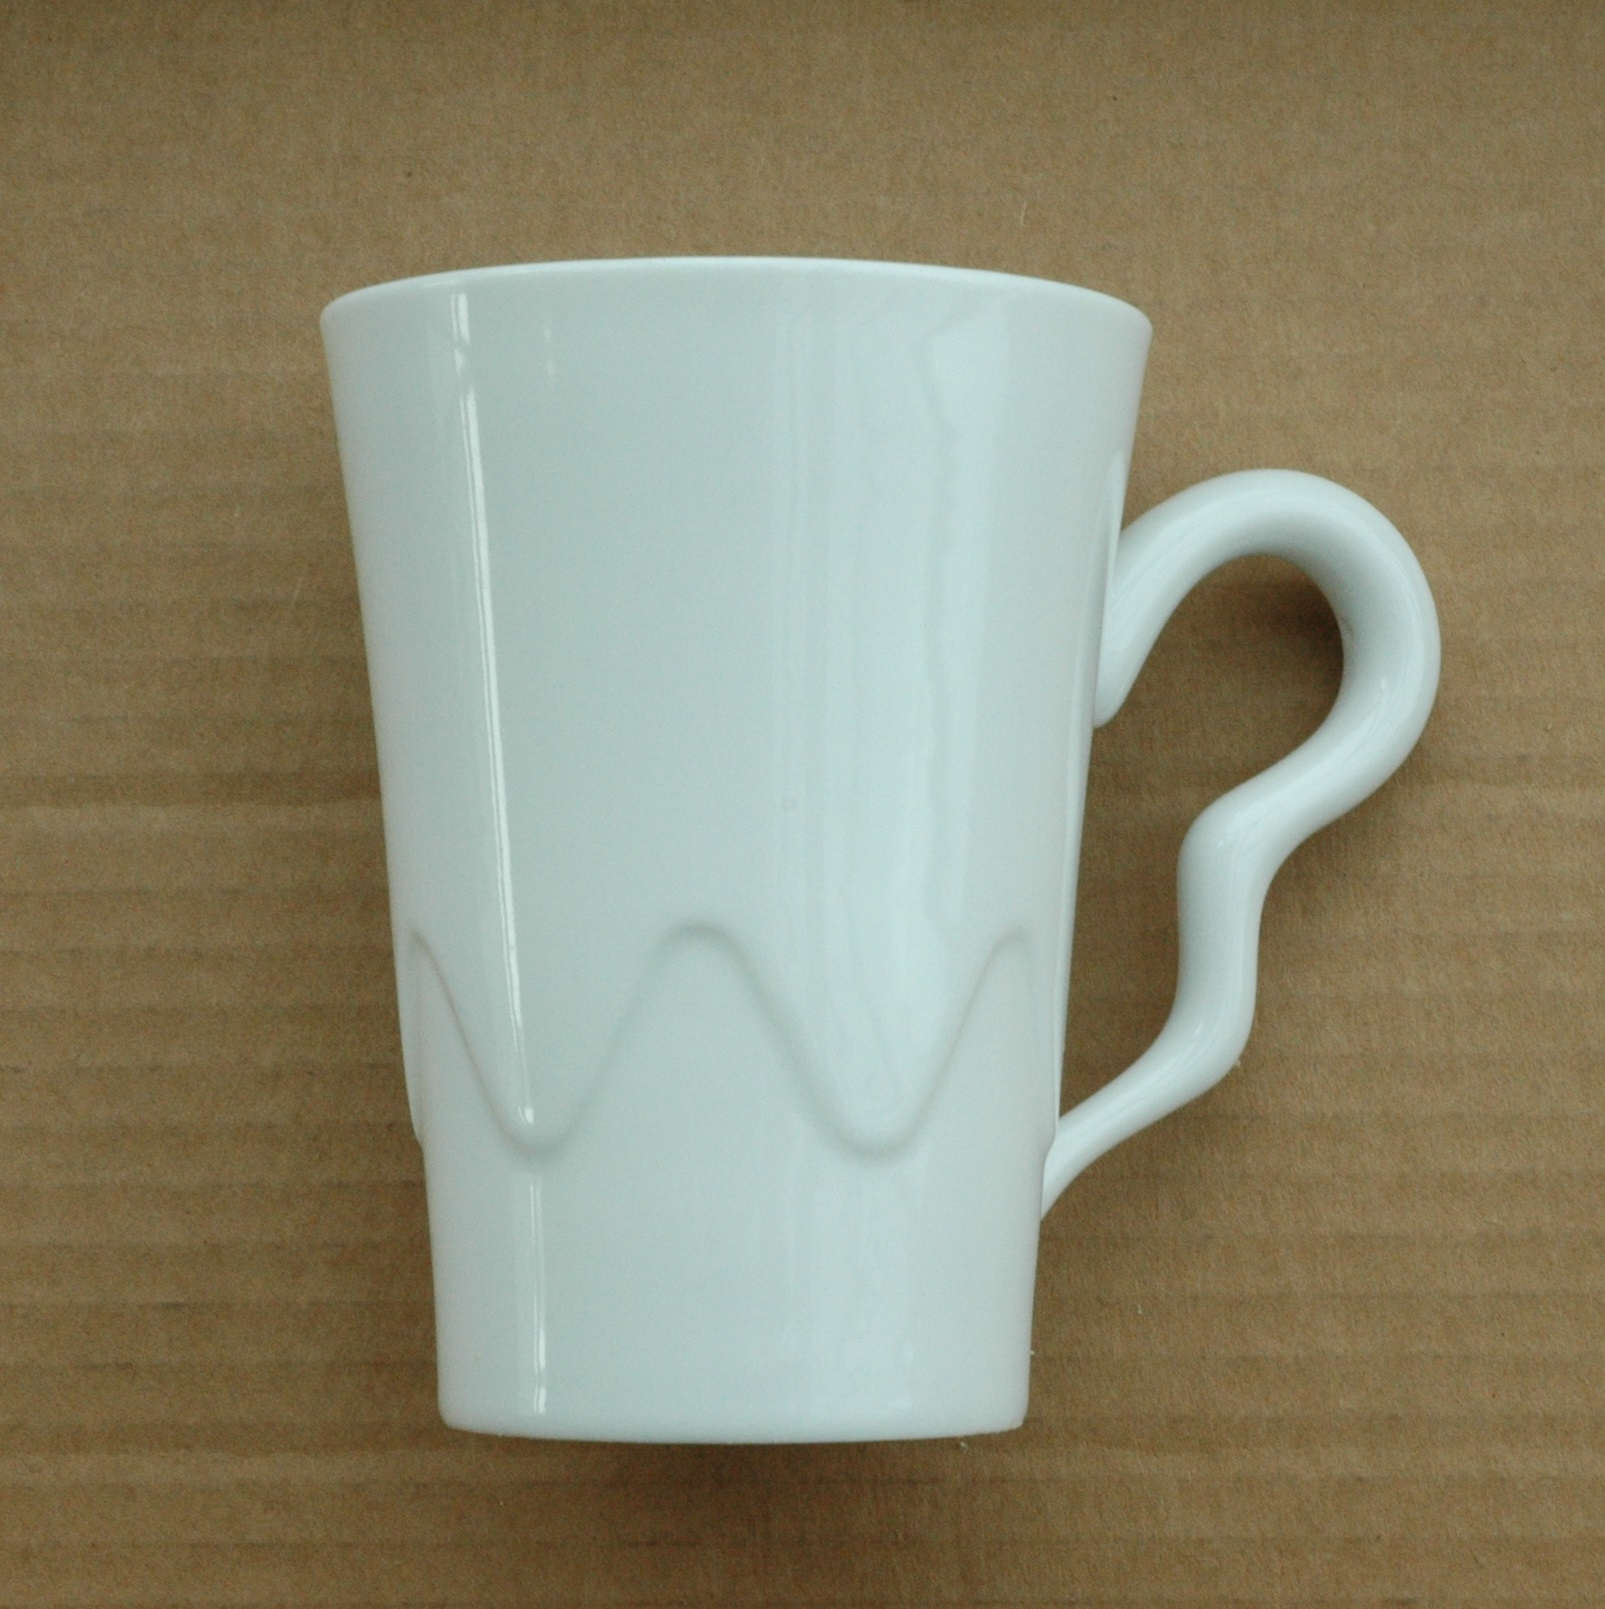
\includegraphics[width=0.15\textwidth]{interp/real_world_img/cup/cup} &
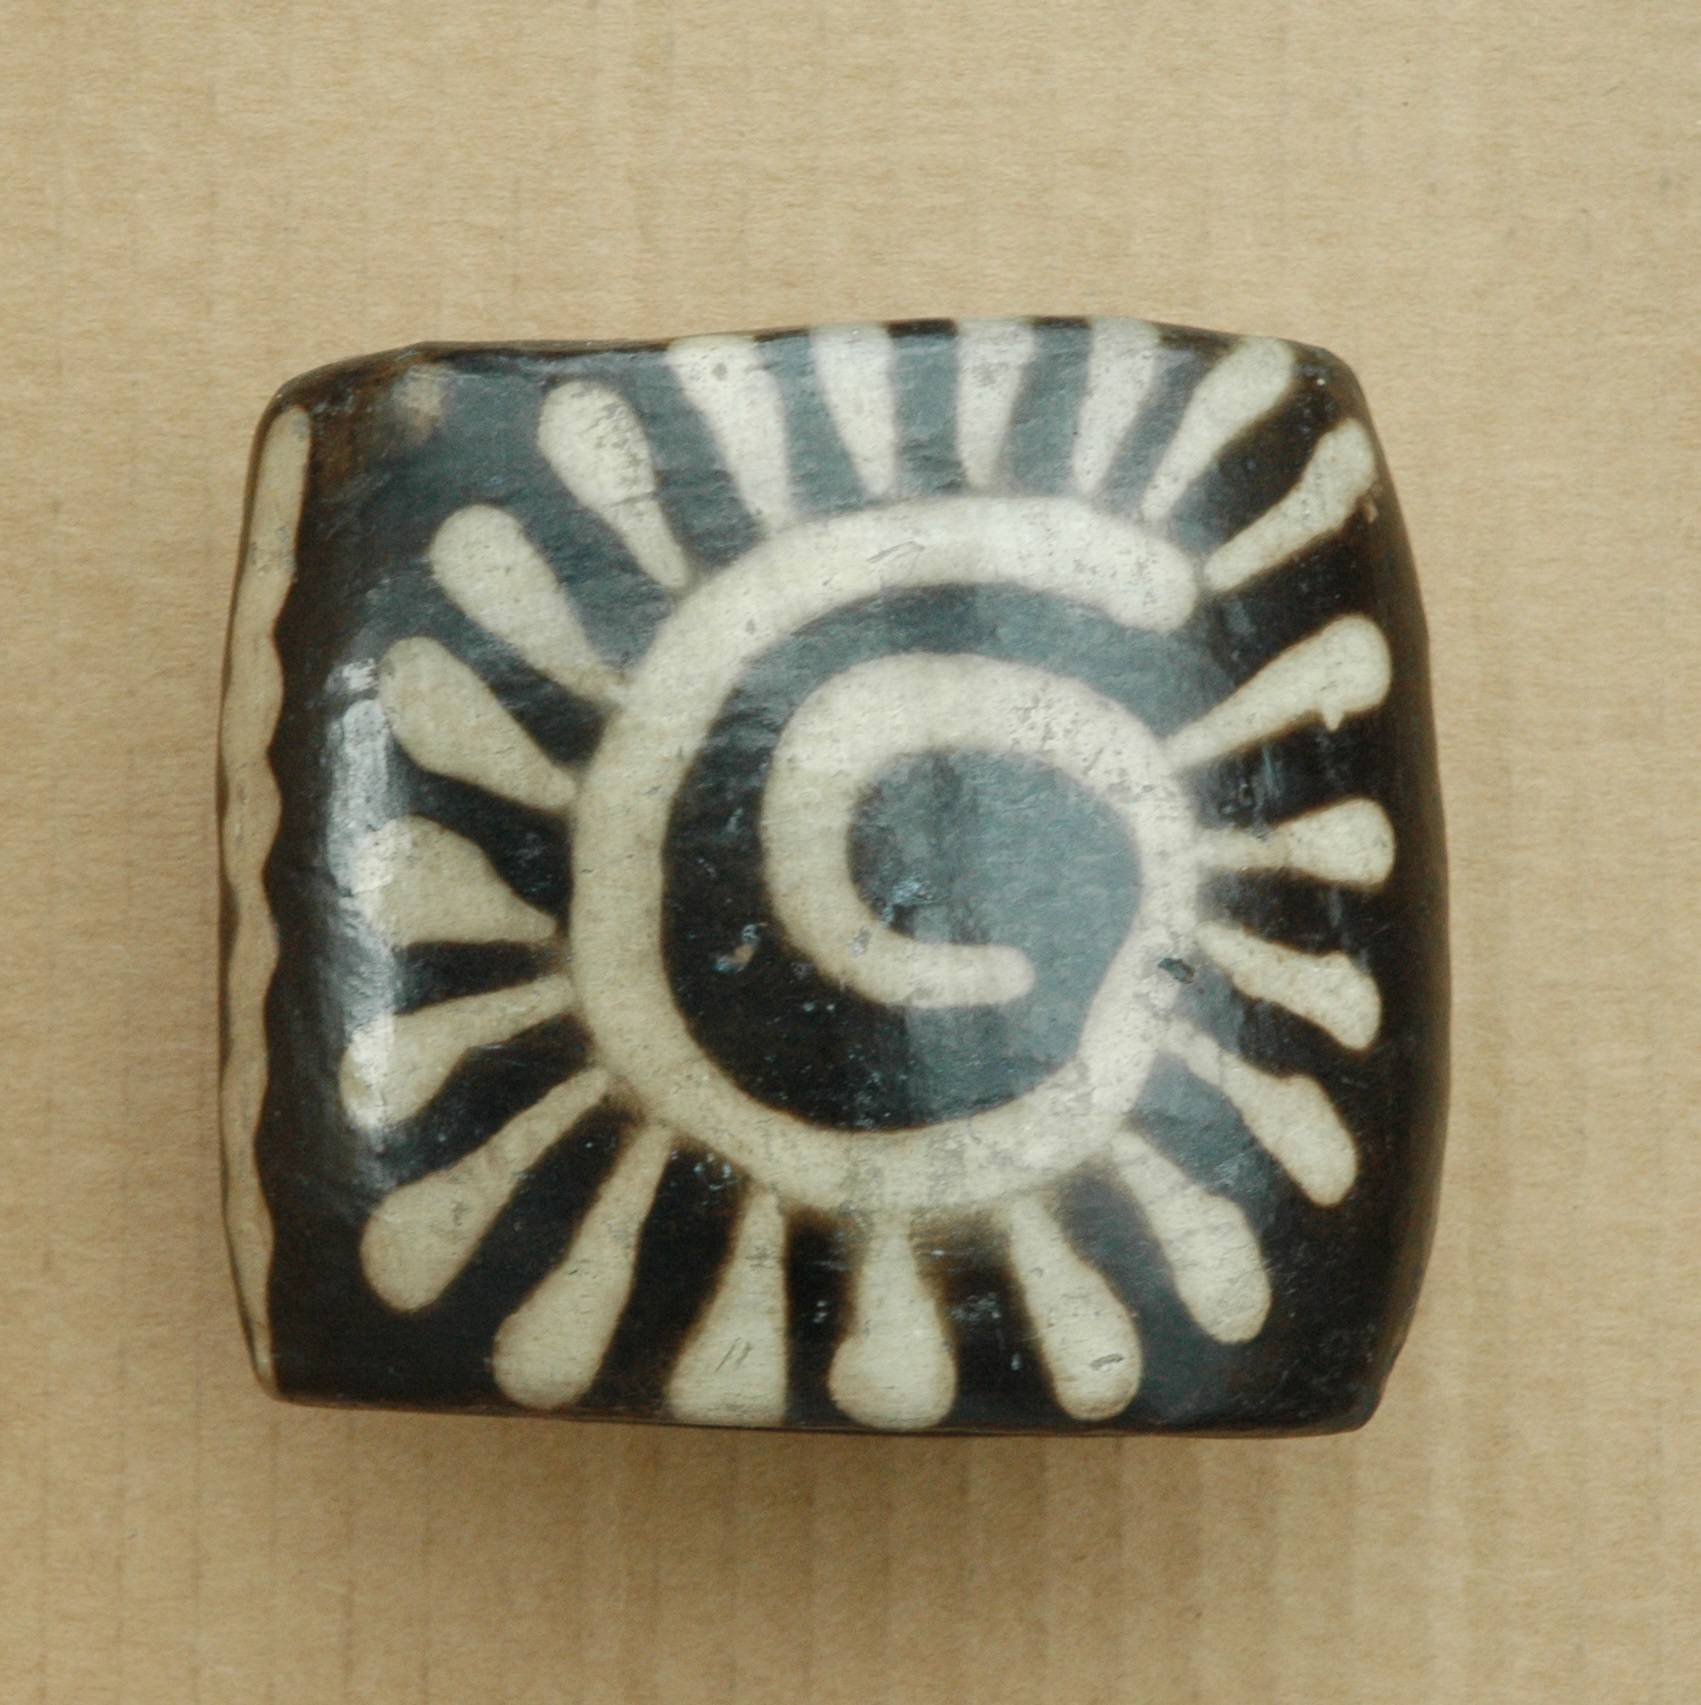
\includegraphics[width=0.15\textwidth]{interp/real_world_img/pot/pot} &
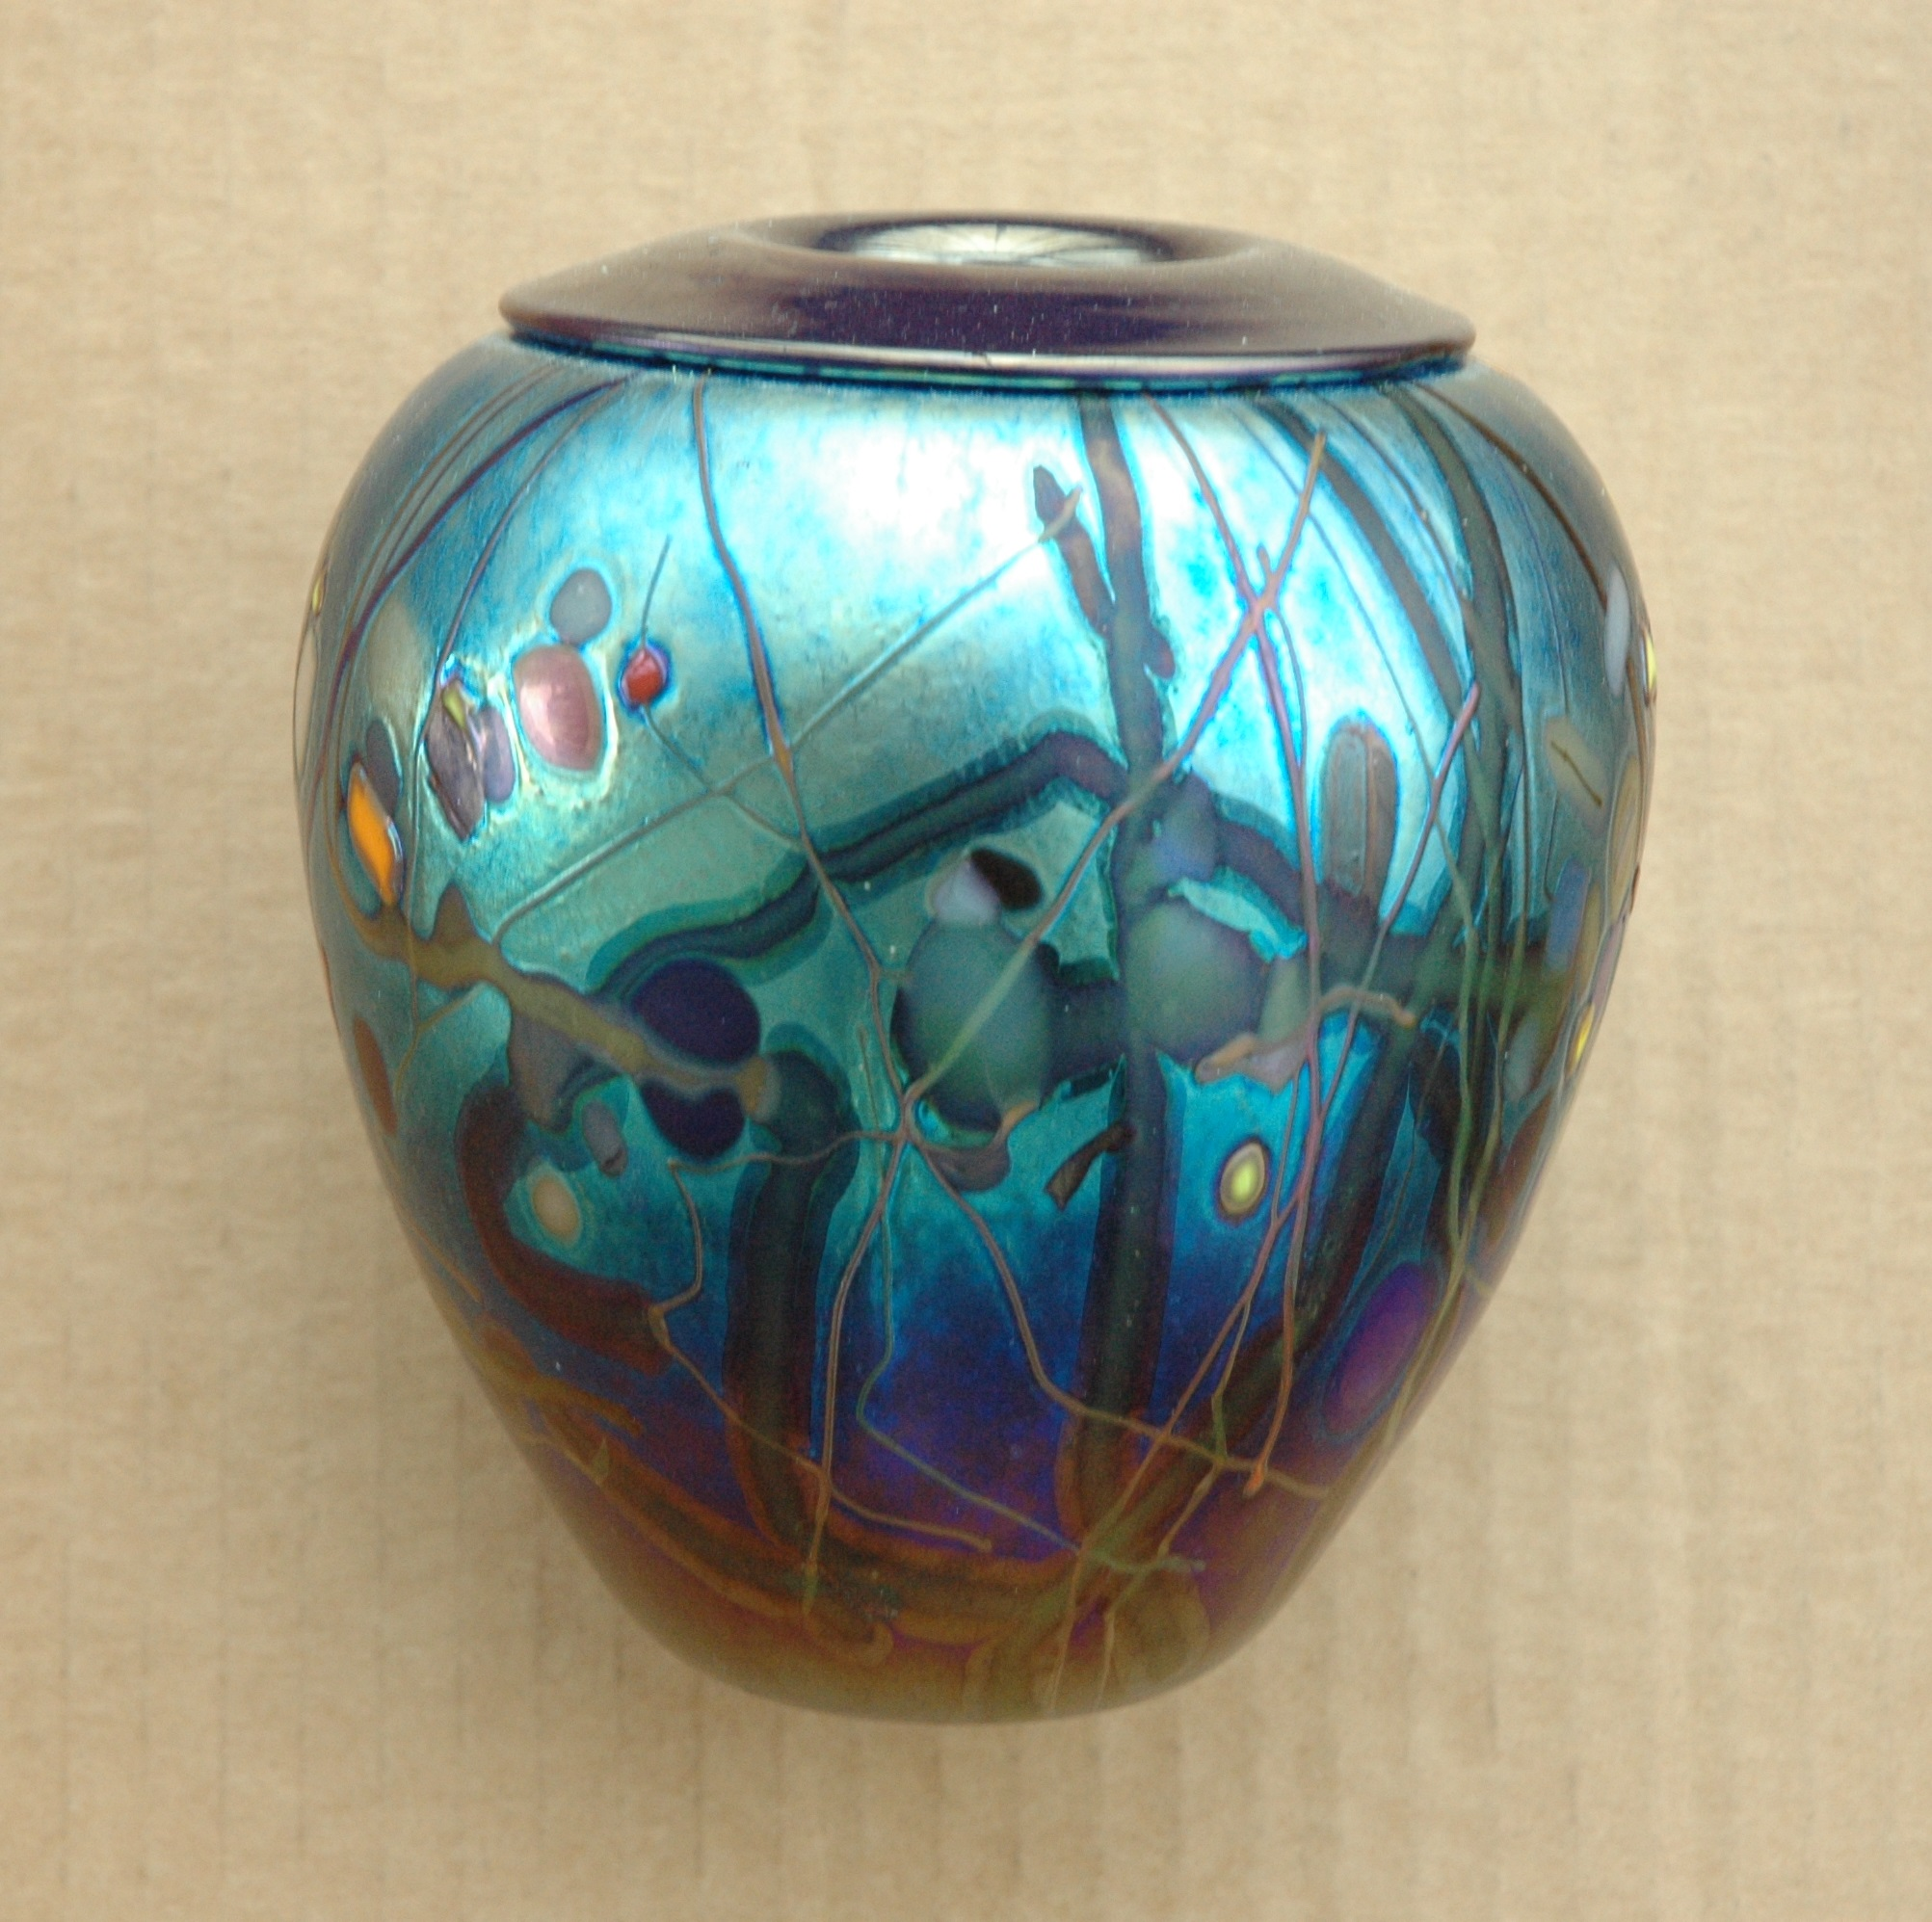
\includegraphics[width=0.15\textwidth]{interp/real_world_img/vase/vase}
% \\ \cline{1-5}
% \multirow{3}{*}{\rotatebox[origin=c]{90}{appearance}}
%   & textureless & textureless & textured & textured\\
%   & diffuse & mixed d/s & diffuse & mixed d/s\\
%   & bright & bright & bright/dark & bright/dark\\
\end{tabular}
\end{figure}

\end{frame}

%------------------------------------------------
\begin{frame}{Interpretation: accurate description, successful result}

\addtolength{\tabcolsep}{-3pt}
\begin{figure}
\centering
\begin{tabular}{*{8}{p{1cm}}}

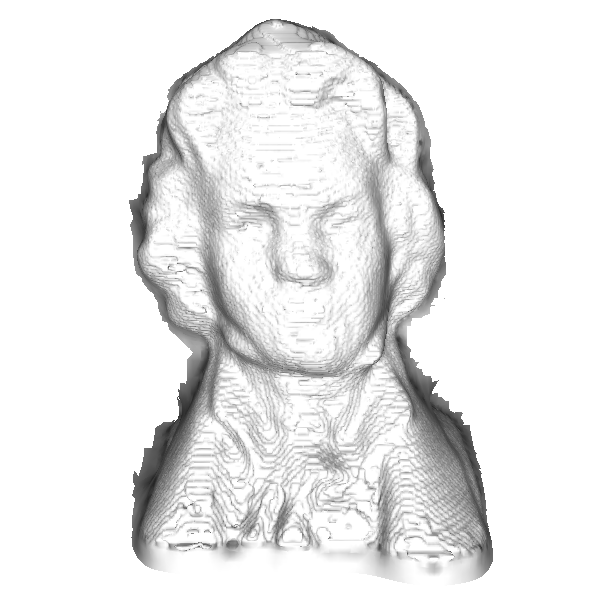
\includegraphics[width=0.12\textwidth]{interp/synth_interp/beethoven_sl} & 
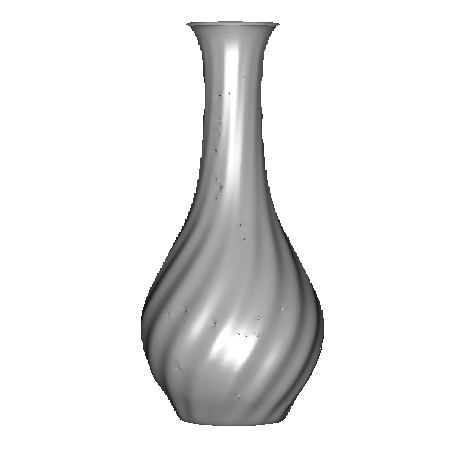
\includegraphics[width=0.12\textwidth]{interp/synth_interp/vase0_ps} &
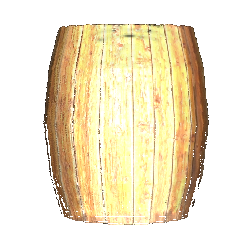
\includegraphics[width=0.12\textwidth]{interp/synth_interp/barrel_sl} &
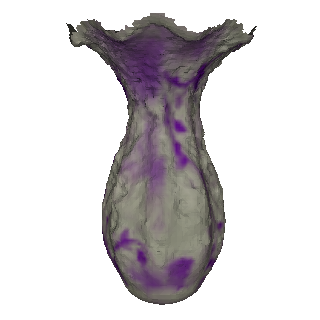
\includegraphics[width=0.12\textwidth]{interp/synth_interp/vase1_mvs} & 
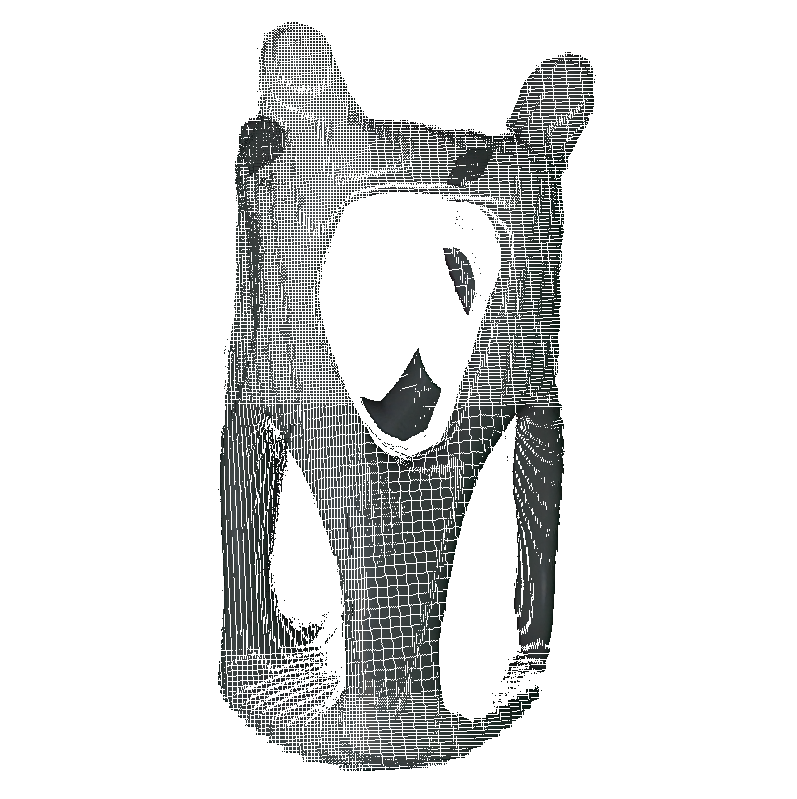
\includegraphics[width=0.12\textwidth]{interp/real_interp/statue/statue_sl} &
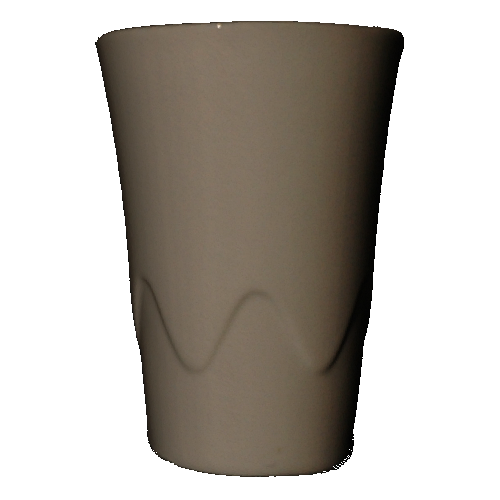
\includegraphics[width=0.12\textwidth]{interp/real_interp/cup/cup_ps} &
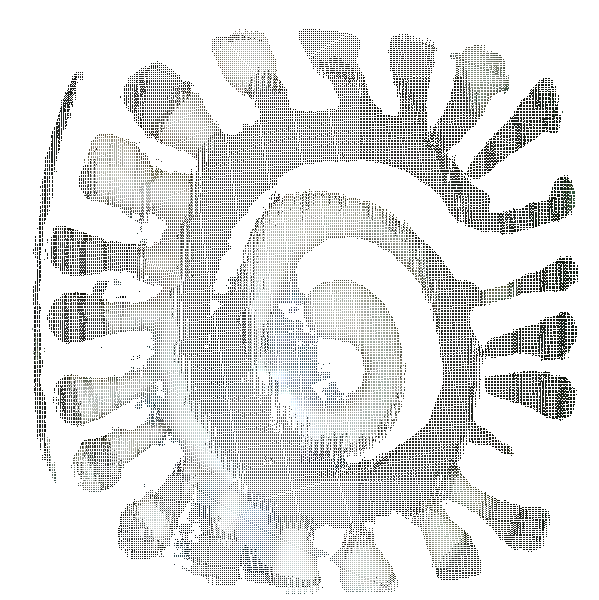
\includegraphics[width=0.12\textwidth]{interp/real_interp/pot/pot_sl} &
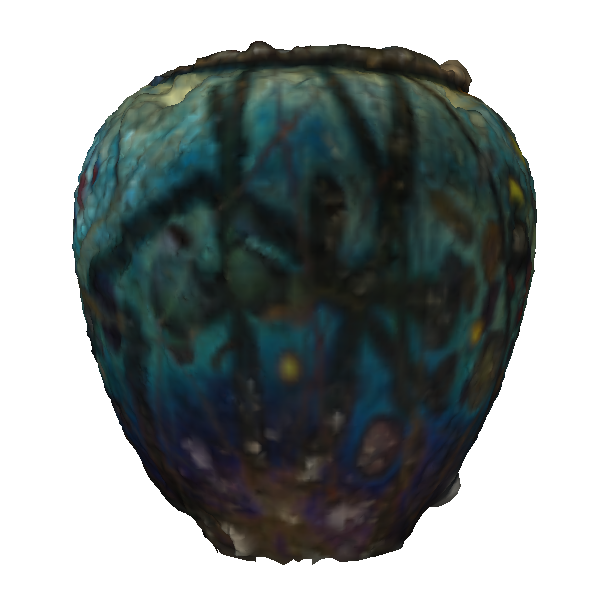
\includegraphics[width=0.12\textwidth]{interp/real_interp/vase/vase_mvs} \\
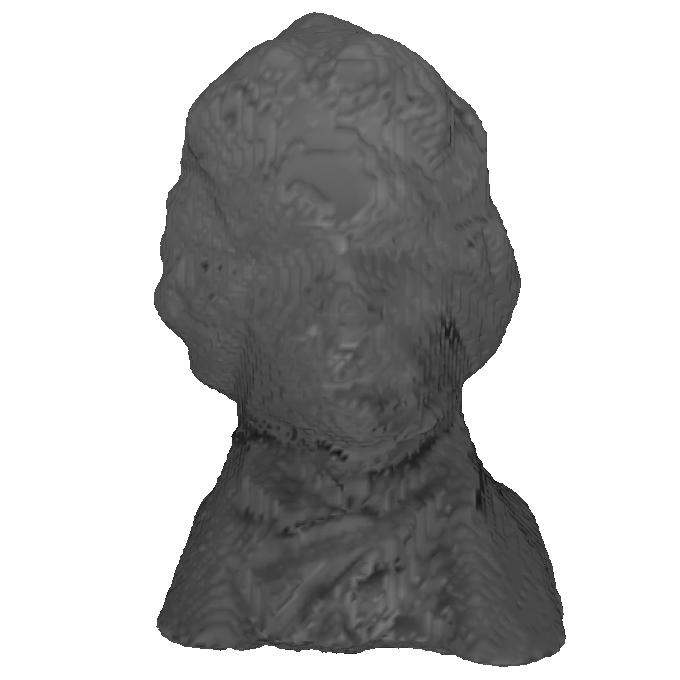
\includegraphics[width=0.12\textwidth]{interp/synth_interp/beethoven_vh} &
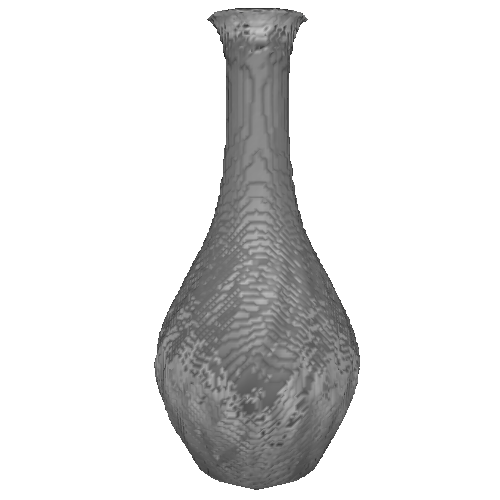
\includegraphics[width=0.12\textwidth]{interp/synth_interp/vase0_vh} &
\includegraphics[width=0.12\textwidth]{interp/synth_interp/barrel_vh} &
\includegraphics[width=0.12\textwidth]{interp/synth_interp/vase1_vh} &
\includegraphics[width=0.12\textwidth]{interp/real_interp/statue/statue_sc} &
\includegraphics[width=0.12\textwidth]{interp/real_interp/cup/cup_sc} &
\includegraphics[width=0.12\textwidth]{interp/real_interp/pot/pot_sc} &
\includegraphics[width=0.12\textwidth]{interp/real_interp/vase/vase_sc} \\

\end{tabular}
\end{figure}
\addtolength{\tabcolsep}{3pt}

\begin{exampleblock}{}
\begin{itemize}
\item accuracy: smoother surface, higher quality
\item completenss: no surface holes
\end{itemize}
\end{exampleblock}

\end{frame}

%------------------------------------------------
\begin{frame}{Interpretation: less accurate description, less successful result}

\addtolength{\tabcolsep}{-6pt}
\begin{figure}
\centering
\begin{tabular}{*{5}{c}|*{5}{c}}
\tc{T}ASR & T\tc{A}SR & TA\tc{S}R & TAS\tc{R} & TASR & \tc{T}ASR & T\tc{A}SR & TA\tc{S}R & TAS\tc{R} & TASR \\
\midrule
\includegraphics[width=0.1\textwidth]{interp/synth_interp/vase0_mvs} &
\includegraphics[width=0.1\textwidth]{interp/synth_interp/vase0_vh} &
\includegraphics[width=0.1\textwidth]{interp/synth_interp/vase0_sl} &
\includegraphics[width=0.1\textwidth]{interp/synth_interp/vase0_sl} &
\includegraphics[width=0.1\textwidth]{interp/synth_interp/vase0_ps} &
\includegraphics[width=0.1\textwidth]{interp/real_interp/cup/cup_mvs} &
\includegraphics[width=0.1\textwidth]{interp/real_interp/cup/cup_sc} &
\includegraphics[width=0.1\textwidth]{interp/real_interp/cup/cup_sl} &
\includegraphics[width=0.1\textwidth]{interp/real_interp/cup/cup_sl} &
\includegraphics[width=0.1\textwidth]{interp/real_interp/cup/cup_ps} \\

\includegraphics[width=0.1\textwidth]{interp/synth_interp/vase1_ps} &
\includegraphics[width=0.1\textwidth]{interp/synth_interp/vase1_vh} &
\includegraphics[width=0.1\textwidth]{interp/synth_interp/vase1_sl} &
\includegraphics[width=0.1\textwidth]{interp/synth_interp/vase1_sl} &
\includegraphics[width=0.1\textwidth]{interp/synth_interp/vase1_mvs} &
\includegraphics[width=0.1\textwidth]{interp/real_interp/vase/vase_ps} &
\includegraphics[width=0.1\textwidth]{interp/real_interp/vase/vase_sc} &
\includegraphics[width=0.1\textwidth]{interp/real_interp/vase/vase_sl} &
\includegraphics[width=0.1\textwidth]{interp/real_interp/vase/vase_sl} &
\includegraphics[width=0.1\textwidth]{interp/real_interp/vase/vase_mvs}\\

\end{tabular}
\end{figure}
\addtolength{\tabcolsep}{6pt}

\begin{exampleblock}{}
\begin{itemize}
\item accuracy or completeness: poorer, rougher, incomplete surface.
\end{itemize}
\end{exampleblock}

\end{frame}

%------------------------------------------------
\begin{frame}{Interpretation: less accurate description, less successful result (cont'd)}

\addtolength{\tabcolsep}{-6pt}
\begin{figure}
\centering
\begin{tabular}{*{5}{c}|*{5}{c}}
\tc{T}ASR & T\tc{A}SR & TA\tc{S}R & TAS\tc{R} & TASR & \tc{T}ASR & T\tc{A}SR & TA\tc{S}R & TAS\tc{R} & TASR\\
\midrule

\includegraphics[width=0.1\textwidth]{interp/synth_interp/beethoven_sl} &
\includegraphics[width=0.1\textwidth]{interp/synth_interp/beethoven_ps} &
\includegraphics[width=0.1\textwidth]{interp/synth_interp/beethoven_sl} &
\includegraphics[width=0.1\textwidth]{interp/synth_interp/beethoven_sl} &
\includegraphics[width=0.1\textwidth]{interp/synth_interp/beethoven_sl} &
\includegraphics[width=0.1\textwidth]{interp/real_interp/statue/statue_sl} &
\includegraphics[width=0.1\textwidth]{interp/real_interp/statue/statue_ps} &
\includegraphics[width=0.1\textwidth]{interp/real_interp/statue/statue_sl} &
\includegraphics[width=0.1\textwidth]{interp/real_interp/statue/statue_sl} &
\includegraphics[width=0.1\textwidth]{interp/real_interp/statue/statue_sl} \\

\includegraphics[width=0.1\textwidth]{interp/synth_interp/barrel_sl} &
\includegraphics[width=0.1\textwidth]{interp/synth_interp/barrel_mvs} &
\includegraphics[width=0.1\textwidth]{interp/synth_interp/barrel_sl} &
\includegraphics[width=0.1\textwidth]{interp/synth_interp/barrel_sl} &
\includegraphics[width=0.1\textwidth]{interp/synth_interp/barrel_sl} &
\includegraphics[width=0.1\textwidth]{interp/real_interp/pot/pot_sl} &
\includegraphics[width=0.1\textwidth]{interp/real_interp/pot/pot_mvs} &
\includegraphics[width=0.1\textwidth]{interp/real_interp/pot/pot_sl} &
\includegraphics[width=0.1\textwidth]{interp/real_interp/pot/pot_sl} &
\includegraphics[width=0.1\textwidth]{interp/real_interp/pot/pot_sl} \\

\end{tabular}
\end{figure}
\addtolength{\tabcolsep}{6pt}

\begin{exampleblock}{}
\begin{itemize}
\item accuracy or completeness: comparable 
\item less accurate descriptions trigger the same algorithm as the accurate one.
\end{itemize}
\end{exampleblock}

\end{frame}

%------------------------------------------------
\begin{frame}{Interpretation: demonstrative result (cont'd)}

\begin{figure}
\centering
\includegraphics[width=\textwidth]{images/interp2_2.pdf}
\end{figure}

\end{frame}

%------------------------------------------------
\begin{frame}{Interpretation: inaccurate description, poor result}

\addtolength{\tabcolsep}{-3pt}
\begin{figure}
\centering
\begin{tabular}{*{8}{p{1cm}}}

\includegraphics[width=0.12\textwidth]{interp/synth_interp/beethoven_vh} &
\includegraphics[width=0.12\textwidth]{interp/synth_interp/vase0_mvs} &
\includegraphics[width=0.12\textwidth]{interp/synth_interp/barrel_vh} &
\includegraphics[width=0.12\textwidth]{interp/synth_interp/vase1_ps} &
\includegraphics[width=0.12\textwidth]{interp/real_interp/statue/statue_sc} &
\includegraphics[width=0.12\textwidth]{interp/real_interp/cup/cup_mvs} &
\includegraphics[width=0.12\textwidth]{interp/real_interp/pot/pot_sc} &
\includegraphics[width=0.12\textwidth]{interp/real_interp/vase/vase_ps} \\

\includegraphics[width=0.12\textwidth]{interp/synth_interp/beethoven_sl} &
\includegraphics[width=0.12\textwidth]{interp/synth_interp/vase0_ps} &
\includegraphics[width=0.12\textwidth]{interp/synth_interp/barrel_sl} &
\includegraphics[width=0.12\textwidth]{interp/synth_interp/vase1_mvs} &
\includegraphics[width=0.12\textwidth]{interp/real_interp/statue/statue_sl} &
\includegraphics[width=0.12\textwidth]{interp/real_interp/cup/cup_ps} &
\includegraphics[width=0.12\textwidth]{interp/real_interp/pot/pot_sl} &
\includegraphics[width=0.12\textwidth]{interp/real_interp/vase/vase_mvs} \\

\end{tabular}
\end{figure}
\addtolength{\tabcolsep}{3pt}

\begin{exampleblock}{}
\begin{itemize}
\item Baseline method is selected by the interface;
\item accuracy or completeness: poor, rougher, incomplete surface.
\end{itemize}
\end{exampleblock}

\end{frame}

%------------------------------------------------
\begin{frame}{Interpreter: demonstrative example}

\setlength{\fboxrule}{2pt}
\addtolength{\tabcolsep}{-3pt}
\begin{figure}
\centering
\begin{tabular}{ccccc}

\includegraphics[width=0.2\textwidth]{images/interp11.pdf} &
\includegraphics[width=0.15\textwidth]{interp/real_interp/statue/statue_mvs} &
\includegraphics[width=0.15\textwidth]{interp/real_interp/statue/statue_ps} &
\fcolorbox{green}{white}{\includegraphics[width=0.15\textwidth]{interp/real_interp/statue/statue_sl}} &
\includegraphics[width=0.15\textwidth]{interp/real_interp/statue/statue_sc} \\

\includegraphics[width=0.2\textwidth]{images/interp12.pdf} &
\includegraphics[width=0.15\textwidth]{interp/real_interp/statue/statue_mvs} &
\includegraphics[width=0.15\textwidth]{interp/real_interp/statue/statue_ps} &
\fcolorbox{green}{white}{\includegraphics[width=0.15\textwidth]{interp/real_interp/statue/statue_sl}} &
\includegraphics[width=0.15\textwidth]{interp/real_interp/statue/statue_sc} \\

\includegraphics[width=0.2\textwidth]{images/interp13.pdf} &
\includegraphics[width=0.15\textwidth]{interp/real_interp/statue/statue_mvs} &
\includegraphics[width=0.15\textwidth]{interp/real_interp/statue/statue_ps} &
\fcolorbox{green}{white}{\includegraphics[width=0.15\textwidth]{interp/real_interp/statue/statue_sl}} &
\fcolorbox{red}{white}{\includegraphics[width=0.15\textwidth]{interp/real_interp/statue/statue_sc}} \\

\end{tabular}
\end{figure}

\end{frame}

%------------------------------------------------
\begin{frame}{Interpreter: demonstrative example}

\setlength{\fboxrule}{2pt}
\addtolength{\tabcolsep}{-3pt}
\begin{figure}
\centering
\begin{tabular}{ccccc}

\includegraphics[width=0.2\textwidth]{images/interp21.pdf} &
\includegraphics[width=0.15\textwidth]{interp/real_interp/cup/cup_mvs} &
\fcolorbox{green}{white}{\includegraphics[width=0.15\textwidth]{interp/real_interp/cup/cup_ps}} &
\includegraphics[width=0.15\textwidth]{interp/real_interp/cup/cup_sl} &
\includegraphics[width=0.15\textwidth]{interp/real_interp/cup/cup_sc} \\

\includegraphics[width=0.2\textwidth]{images/interp22.pdf} &
\fcolorbox{red}{white}{\includegraphics[width=0.15\textwidth]{interp/real_interp/cup/cup_mvs}} &
\fcolorbox{green}{white}{\includegraphics[width=0.15\textwidth]{interp/real_interp/cup/cup_ps}} &
\includegraphics[width=0.15\textwidth]{interp/real_interp/cup/cup_sl} &
\includegraphics[width=0.15\textwidth]{interp/real_interp/cup/cup_sc} \\

\includegraphics[width=0.2\textwidth]{images/interp23.pdf} &
\fcolorbox{red}{white}{\includegraphics[width=0.15\textwidth]{interp/real_interp/cup/cup_mvs}} &
\fcolorbox{green}{white}{\includegraphics[width=0.15\textwidth]{interp/real_interp/cup/cup_ps}} &
\includegraphics[width=0.15\textwidth]{interp/real_interp/cup/cup_sl} &
\includegraphics[width=0.15\textwidth]{interp/real_interp/cup/cup_sc} \\

\end{tabular}
\end{figure}

\end{frame}

\end{document}